\documentclass{article}
\usepackage[utf8]{inputenc}
\usepackage{graphicx}
\usepackage[margin=1.0in]{geometry}
\usepackage{float}
\usepackage{wrapfig}
\usepackage{textcomp}
\usepackage{mathtools, nccmath}
\usepackage{amssymb}
\usepackage{amsmath}
\usepackage{mathrsfs}
\usepackage{dsfont}
\usepackage{lmodern}
\usepackage{textcomp}
\usepackage{hyperref}
\usepackage{physics}
\usepackage{listings}
\setlength{\parindent}{0pt}
\usepackage{setspace}
\usepackage[sorting=none]{biblatex}
\usepackage{caption}
\usepackage{subcaption}
\usepackage[eng]{nbi}
%\addbibresource{lit.bib}
\onehalfspacing

\supervisor{Klaus Mølmer}
\project{Project outside course scope}
\author{Emil H. Henningsen}
\title{Investigation of Collective Atomic Excitation States}
\subtitle{}
\institute{Niels Bohr Institute}
\department{Hy-Q - Center for Hybrid Quantum Networks}
\email{tzs820@alumni.ku.dk}
\handindate{$14^{th}$ of June, 2024}
\defencedate{$21^{st}$ of June, 2024}

\begin{document}

\maketitle

\section*{Abstract}

TODO. 

\section*{Acknowledgements}

\newpage
\tableofcontents

\section{Introduction}

The collective excitation states of an atomic array is a well-known phenomenon in the physics of light-matter interaction (REF). In the field of quantum information processing, long-lived quantum states are desired for implementing both quantum communication protocols and quantum computing. Certain excited states of atomic arrays display greatly amplified (superradiant) or suppresed (subradiant) decay rates, when compared to a single atom in vacuum. Such states arise in the interplay of atoms arranged closely together and the surrounding electromagnetic field. In the following, exciting new geometries and variations are investigated within the scope of finding highly subradiant states. The model used for these calculations is a second quantized approach, in which the atoms are assumed dipoles, and the suppresed radiance is manifested as destructive interference between these (???). Furthermore, theoretical considerations are presented to elaborate on expectations and results of these calculations. This project is restricted to radiation in free-space. 

Hvad er mine quantities of interest?

\section{Theory}\label{sec:theory}

The model is developed from a classical perspective, but will in the end be used to describe the quantized field and therefore be a fully quantum model (REF Gruner og Welsch). The model is used to describe the interaction between atoms and the empty-space electromagnetic field. The model is capable of describing both homogenous and inhomogenous Kramers-Kronig dielectrics (REF Gruner og Welsch), which makes it desirable for in-depth studies of collectively excited atomic arrays in various settings and environments. Due to the quantities of interest in this project, the framework is restricted to free space in the following. 

List of assumptions and approximations (REF Asenjo):
\begin{itemize}\label{list:assumptions}
    \item All photons are mediated in vacuum, i.e. $\varepsilon(\bar{r},\omega) = \varepsilon_0$,
    \item Targeting a single transition in the atoms (two-level system), the dipole-interaction between atoms and the field happens at a narrow band-width, i.e. $\omega \rightarrow \omega_0$,
    \item The atoms are tightly trapped, such that their positions can be treated as stationary points. 
    \item Interatomic distances are smaller than the wavelength of emitted photons, $d < \lambda_0$. With this, the retardation of the field between the atoms can be neglected, 
    \item There are no strongly-coupled modes between the field and the atoms (which would e.g. be the case, if the atoms were placed in an optical cavity). Together with the abovementioned assumption, the emission is in the Markovian regime, which means "the system will have no memory of its past" (REF Deutsch) once the photon has escaped. 
\end{itemize}
The latter two points allow for the promotion of field and dipole moment to quantum operators, after which the field described by Green's tensor and radiation-scattering dipoles can be coherently described by atomic coherence operators. In particular, the Green's tensor under these assumptions become (REF Asenjo, Equation 6):

\begin{equation}\label{eq:Greens}
    \underline{G}_0 (\bar{r}_{ij}, \omega_0) = \frac{e^{ik_0r}}{4\pi k_0^2 r^3} \cdot \left[ (k_0^2r^2 + ik_0r - 1) \mathds{1}_3 + (-k_0^2 r^2 -3ik_0r + 3) \frac{\ket{\bar{r}_{ij}}\bra{\bar{r}_{ij}}}{r^2} \right].
\end{equation}
Where $r$ is the norm of the displacement between atoms i and j: $\bar{r}_{ij}$, $k_0=\frac{\omega_0}{c}$ is the norm of the wave vector, $\mathds{1}_3$ is the three-dimensional identity matrix and $\ket{\bar{r}_{ij}}\bra{\bar{r}_{ij}}$ is the outer product of the displacement vector. 

The effective Hamiltonian (REF Asenjo), which is subject to diagonalization:
\begin{equation}\label{eq:Heff}
    \begin{split}
        \hat{H}_{eff} &= - \mu_0 \cdot \omega_0^2 \cdot \sum_{i,j = 1}^N \bar{\mathscr{D}}^\dagger \underline{G}_0(\bar{r_i}, \bar{r_j}, \omega_0) \bar{\mathscr{D}} \sigma_+^i \sigma_-^j, \\
        &=- \mu_0 \cdot \omega_0^2 \cdot \|\bar{\mathscr{D}}\|^2 \cdot \sum_{i,j = 1}^N \hat{n}^T \underline{G}_0(\bar{r_i}, \bar{r_j}, \omega_0) \hat{n} \sigma_+^i \sigma_-^j. \\
    \end{split}
\end{equation}
Where $\mu_0$ is the vacuum permeability, $\omega_0$ is the atomic transition frequency, $\bar{\mathscr{D}}$ is the dipole vector at atom j (however, for most applications, equal directioned dipoles are chosen) and $\sigma_\pm^i$ is the i'th atom's coherence operators acting on the i'th subspace of full Hilbert space. In the last line, the dipole amplitude is separated from the direction, which proves useful when converting to a dimensionless model in Section \ref{sec:dimless}. This matrix fully describes the atom-atom interaction in a quantum jump formalism (REF Asenjo). However, this is not the entire description of the system. At some point, a photon mode is excited, and the excitation is lost to the system. This reflects in the fact that the above matrix is non-Hermitian, i.e. $\hat{H}_{eff} \neq \hat{H}_{eff}^\dagger$. Hermitian matrices conserve norm, meaning no probability amplitude leaves the system. In this description, probability amplitude "leaks" away, as the probability of exciting a photon mode increases (this is elaborated more in Section \ref{sec:full_system}). If the system is initialized with an excitation, then at $t=0$, the eigenvectors are the actual eigenstates of the system, even though the non-Hermiticity dictates the non-existence of a single orthonormal basis for the singular value decomposition. It is therefore still valid to consider the eigenvectors, and of particular interest in this project the eigenvalues, of the effective Hamiltonian. The eigenvalues of this matrix are complex numbers, where the real part corresponds to a finite energyshift due to the atoms being close together, and the imaginary part corresponds to damping in time of the state, i.e. decay rates (REF Asenjo, Equation 7): $\lambda_\xi = J_\xi - \frac{i}{2} \Gamma_\xi$. The steps taken towards diagonalizing the matrix is described in Section \ref{sec:block}. 

Another issue must also be adressed before working with the abovementioned framework. It is evident in Equation \ref{eq:Greens} that the diagonal values diverge, when the distance goes to zero. The diagonal values describe the interaction of the atoms with themselves, i.e. if they were to be alone, $N = 1$, there should be no energy shift, and the decay rate must be the well-known spontaneous vacuum emission rate:

\begin{equation}\label{eq:vac_emission_rate}
    \Gamma_0 = \frac{\omega_0^3}{3\pi \hbar \varepsilon_0 c^3} \cdot \|\bar{\mathscr{D}}\|^2
\end{equation}

Therefore, the diagonal values of $\hat{H}_{eff}$ are but a constant offset of the identity, which gives the full matrix:

\begin{equation}
    \hat{H} = \sum_{i=0}^N (\hbar \omega_0 - \frac{i}{2}\Gamma_0) \hat{\sigma}_{ee}^{i} -\mu_0 \omega_0^2 \|\bar{\mathscr{D}}\|^2 \sum_{i,j = 1, i \neq j}^N \hat{n}^T \underline{G}_0(\bar{r}_{ij}, \omega_0) \hat{n} \sigma_+^i \sigma_-^j.
\end{equation}
NOTE: Ved ikke lige med denne del.... Skal i hvert fald inkludere noget omkring diagonalen indsættes ved håndkraft.

In general, becuase the atomic transitions are well-defined two-level systems, this formalism can be considered as spin-wave excitations in arrays of spin-½ particles. This does not give any more clarity on the behaviour of the system for single excitation states, as this is equivalently described by interference between the dipoles. It is another case, when considering multiple excitation states, as the fermionic nature of spin-½ particles gives rise to interesting dynamics (REF Asenjo, Section IIIC). In this project, the quantities of interest limits the use of the formalism to the single-excitation manifold, but multiple excitations is one of the directions outlined as further research in Section \ref{sec:further}. 

Kæde: Foton kan ikke undslippe ortogonalt til kæden. Hvorfor? -> "Spin-bølge" tilstand i gitteret. -> faststoffysik-sprog. Subradiante tilstande for bølgevektorer indenfor første Brillouin-zone. 

Dipolbilledet bliver ukorrekt for to excitationer og derover, men formalismen holder stadig. 

Forudsigelser for N=2 tilfælde? Problemer! Sammenligning med Adrian N=3 kæde. Vidde på egenværdier gør det svært for algoritmen at være præcis, derfor skal der ikke så meget til, før vi havner på den forkerte side.  DISKUSSION?

\subsection{The full system}\label{sec:full_system}
In this section, some justification for the use of the non-Hermitian $\hat{H}_{eff}$ is provided. It is not rigorous for the multiple atoms case, but covers the single atom case, and it is assumed to be a similar relation for multiple atoms. 

A fundamentality of Quantum Mechanics is the unitary evolution of quantum systems. In other words, probability does not "leak" or suddenly increase, but must always sum up to one. For the time-wise propagation of a Hamiltonian to be unitary, the Hamiltonian must be Hermitian, i.e. $\hat[H] = \hat{H}^\dagger$:
\begin{equation}\label{eq:unitarity}
    \hat{U}(t) = e^{i \hat{H} t} \rightarrow \hat{U}(t) \hat{U}^\dagger(t) = e^{i \hat{H} t} e^{-i \hat{H}^\dagger t} = e^{i(\hat{H}-\hat{H}^\dagger) t} = e^{i \underline{0} t} = \mathds{1}.
\end{equation}
Therefore, to truly describe the evolution of the quantum system in question, it must be expanded to include whereever the the probability may go / come from. For the atomic dipoles interacting with the surrounding field, this is in the coupling to a photon mode, as seen in (REF Mølmer og Castin). The full description of the wave function includes the Hilbert space of photon modes, $\mathscr{H} = \mathscr{H}_{atomic} \otimes \mathscr{H}_{photon}$:
\begin{equation}\label{eq:full_wave_function}
    \ket{\psi(t)} = a(t) \ket{g, 0} \sum_{j=1}^N c_j(t) \ket{e_j, 0} + \sum_{\bar{k},s} b_{\bar{k},s} (t) \ket{g, 1_{\bar{k},s}}.
\end{equation}
As noted in (REF Mølmer og Castin), under appropriate assumptions, the evolution of this wavefunction may equally as well be treated by Monte-Carlo simulation. With a certain proability, a quantum jump from excited atomic state to ground state plus a photon has happened. For a single atom, this probability is $\delta p = \Gamma |b(t)|^2 dt$, where $b(t)$ is the probability amplitude of being in the atomic excited state (the $c_j (t)$ in multiple atom case). The probability for a quantum jump to occur in the multiple atom case is not simply this, but it does provide an insight: The non-Hermitian evolution of the system provides the true dynamics, except for the atoms becoming deexcited and the photon leaving the system. 

\subsection{The case of $N=2$}\label{sec:N2}

\begin{equation}\label{eq:N2_general}
    \hat{H}_{eff} = 
    \begin{pmatrix}
        0 & 0 & 0 & 0 \\
        0 & \hbar \omega_0 & 0 & 0 \\
        0 & 0 & \hbar \omega_0 & 0 \\
        0 & 0 & 0 & 2 \hbar \omega_0 \\
    \end{pmatrix}
    - \mu_0 \omega_0^2 \| \bar{\mathscr{D}} \|^2
    \begin{pmatrix}
        0 & 0 & 0 & 0 \\
        0 & h_{11} & h_{12} & 0 \\
        0 & h_{21} & h_{22} & 0 \\
        0 & 0 & 0 & h_{11} + h_{22} \\
    \end{pmatrix}
\end{equation}
Where $h_{ij}$ is the matrix element $\hat{n}^T G_0(\bar{r}_{ij},\omega_0) \hat{n}$. As discussed, the diagonal values are due to the interaction of the atoms with themselves, i.e. it is the spontaneous decay rate. The analytical $N=2$ case show an important property of the Hamiltonian structure, which will be utilized for the analysis of larger systems in Section \ref{sec:block}. The Hamiltonian is block diagonal, meaning its entries are collected in blocks of excitation number. DIAGONALIZE 2x2 matrix. Story about negative decay rates. Succes? Is the Green's tensor the appropriate form for this problem? Can we still rely on the Markov regime, when $r->0$ ? By then, the energyshift becomes cubic inverse bigger, which may take omega out of the range of Markov.

\subsection{Time-evolution of excitation}\label{sec:time-evolution}

In this section, it is briefly introduced how to compute the time-evolution of an excitated state of the efficient Hamiltonian. Unfortunately, the there was not enough time in this project to perform a detailed analysis of the time-evolution of the different states. However, the theoretical section is still included for completeness.

The effective Hamiltonian has no time-dependency, and it is therefore possible to evolve the states according to Schrödinger's equation. An expansion of a state into the eigenstates of the effective Hamiltonian including the wiggle-factors of corresponding eigenvalues (including both energyshift and damping) yields the apparent evolution:

\begin{equation}
    \begin{split}
        \ket{\psi (t)} = \sum_{\xi=1}^N c_\xi \ket{\psi_\xi} e^{i \lambda_\xi t}
    \end{split}
\end{equation}

\section{Method}

Issue: Full size of Hilbert-space scales exponentially -> high memory requirements.

Many-body quantum mechanics is in many cases a challenge to compute. In this case, the goal is to find the eigenvalues and eigenvectors of the Hamiltonian in Equation \ref{eq:Heff}. Diagonalization of a matrix is a computation in polynomial time of the dimension, but since the Hamiltonian encodes the information of an exponentially increasing dimensional Hilbert-space, the scaling of the diagonalization algorithm is exponential in system size. Furthermore, the memory requirements for storing the Hamiltonian is also exponentially increasing for every atom that is added to the system. Also for sparse matrix methods. Therefore, it is not tractable to consider the full Hilbert space, when diagonalizing the Hamiltonian classically. In this section, it is briefly introduced, how the block-structure of the effective Hamiltonian enables diagonalization for a (relatively) low number of excitations. Furthermore, the equations are transformed to unitless equations to better accommodate precision. 

\subsection{Block hamiltonian}\label{sec:block}

The structure of Equation \ref{eq:Heff} has a useful property, as seen initially for the $N=2$ case in Section \ref{sec:N2}. It commutes with the excitation-number operator (FINDES DEN?), $[\hat{H}_{eff}, \hat{N}_{exc}] = 0$, which means the Hamiltonian has a block-diagonal structure. In other words, in the basis of single excitations, the Hamiltonian is effectively an $N \times N$ matrix. The basis is $\{ \ket{e_i} \}_{i=1}^N$, where $\ket{e_i}$ is the i'th atom excited and the remaining in the ground state: $\ket{g_1, g_2, g_3, ..., e_i, ..., g_{N-1}, g_N}$. In the single excitation case, the problem is but the diagonalization of an $N \times N$ matrix. In the k excitations case, it is determined by the binomial factor, because of the two-level nature of the atoms: $\begin{pmatrix} N \\ k \\ \end{pmatrix} \times \begin{pmatrix} N \\ k \\ \end{pmatrix}$. Therefore, it is still not possible to consider a high k (i.e. more than a few), as the binomial factor scales too fast. 

\subsection{Dimensionless computation}\label{sec:dimless}

Finding the eigenvalues of the system is now efficiently solvable in a classical setting. In order to preserve as much precision as possible, the dimensions are transformed to a unitless system. This is done by choosing the following units: $[E]=\hbar \Gamma_0$, $[r] = k_0^{-1}$ and $[t] = \Gamma_0^{-1}$, where $\Gamma_0$ is the vacuum spontaneous emission rate. The choice of units for energy and distance will give the following changes: 

\begin{equation}\label{eq:Green_unitless}
    \begin{split}
        &\underline{G_0}(\bar{r}_{ij}, \omega_0) \longrightarrow k_0 \cdot \tilde{\underline{G}}_0(\bar{\tilde{r}}_{ij}) \\
        \rightarrow &\tilde{\underline{G}}_0(\bar{\tilde{r}}_{ij}) = \frac{e^{i\tilde{r}}}{4\pi \tilde{r}^3} \left[ (\tilde{r}^2 - i\tilde{r} + 1) \mathds{1}_3 (-\tilde{r}^2 - 3i\tilde{r} + 3) \frac{\ket{\bar{\tilde{r}}_{ij}}\bra{\bar{\tilde{r}}_{ij}}}{\tilde{r}^2} \right]
    \end{split}
\end{equation}
Where $\tilde{r}$ is the norm of $\bar{\tilde{r}}_{ij}$. The Green's tensor is now unitless. In order to get the Hamiltonian in the above energy units, a few factors must be considered. The factor in front of $\hat{H}_{eff}$, $A_0$ is after changing units of Green's tensor compared to $\hbar \Gamma_0$, which finally gives the unitless Hamiltonian:

\begin{equation}\label{eq:Hamiltonian_unitless}
    \begin{split}
        &A_0 = -\mu_0 \omega_0^2 \| \bar{\mathscr{D}} \|^2 k_0^{-1} = - \frac{\omega_0^3}{\varepsilon_0 c^3} \| \bar{\mathscr{D}} \|^2 \\
        &\hbar \Gamma_0 = \frac{\omega_0^3}{3\pi \varepsilon_0 c^3} \| \bar{\mathscr{D}} \|^2 \\
        \longrightarrow & \tilde{H}_{ij} = -3 \pi \hat{n}^T \underline{\tilde{G}}_0 (\bar{\tilde{r}}_{ij}) \hat{n}
    \end{split}
\end{equation}
Unless otherwise stated, the above unitless Hamiltonian and variables are the entities in mind, when discussing results, and the tilde's are omitted. 

It is also important to note that the distances inserted the Greens tensor are in units of $2\pi$. $r$ is expressed in units of $k_0^{-1}$, so the actual distance measure is (using $d$ instead of $r$ to distinguish): $\frac{d}{\lambda_0} = 2 \pi r$, which is a useful way to express distances between the atoms, as it compares directly to the wavelength of the photons. 

\section{Results \& Discussion}

Firstly, following (REF Asenjo), the computation is compared to the case of a $N=50$ linear chain with parallel polarized dipoles, i.e. both $\bar{r}_{ij}$ and $\hat{n}$ are directed in the same direction. The results match, and Figure 3 of (REF Asenjo) has been reproduced. Secondly, the variation of polarization in the linear chain is investigated, which may be a particularly relevant parameter, as it is controllable in practice with an external magnetic field. Thirdly, a linear chain broken in the middle with varying angle is investigated to see, how the excitation of the most subradiant mode is spread across the system. Lastly, the circular lattice is also investigated with varying polarizations. Finally, some unexpected negative decay rates are discussed, and some probable causes are proposed. 

\subsection{Linear chain}\label{disc:linear_chain}

In Figure \ref{fig:fig1}, a deeper insight into the linear chain (also referred to as linear lattice) in one dimension. The linear chain is an interesting first geometrical configuration to consider due to its "simplicity". The linear chain introduces less new dependencies to the system and its dynamics. The figure contains both decay rates vs. different variables and the population of the most subradiant states on the chain. 

\begin{figure}[H]
    \centering
    %Figure top left corner
    \begin{subfigure}[b]{0.49\textwidth}
        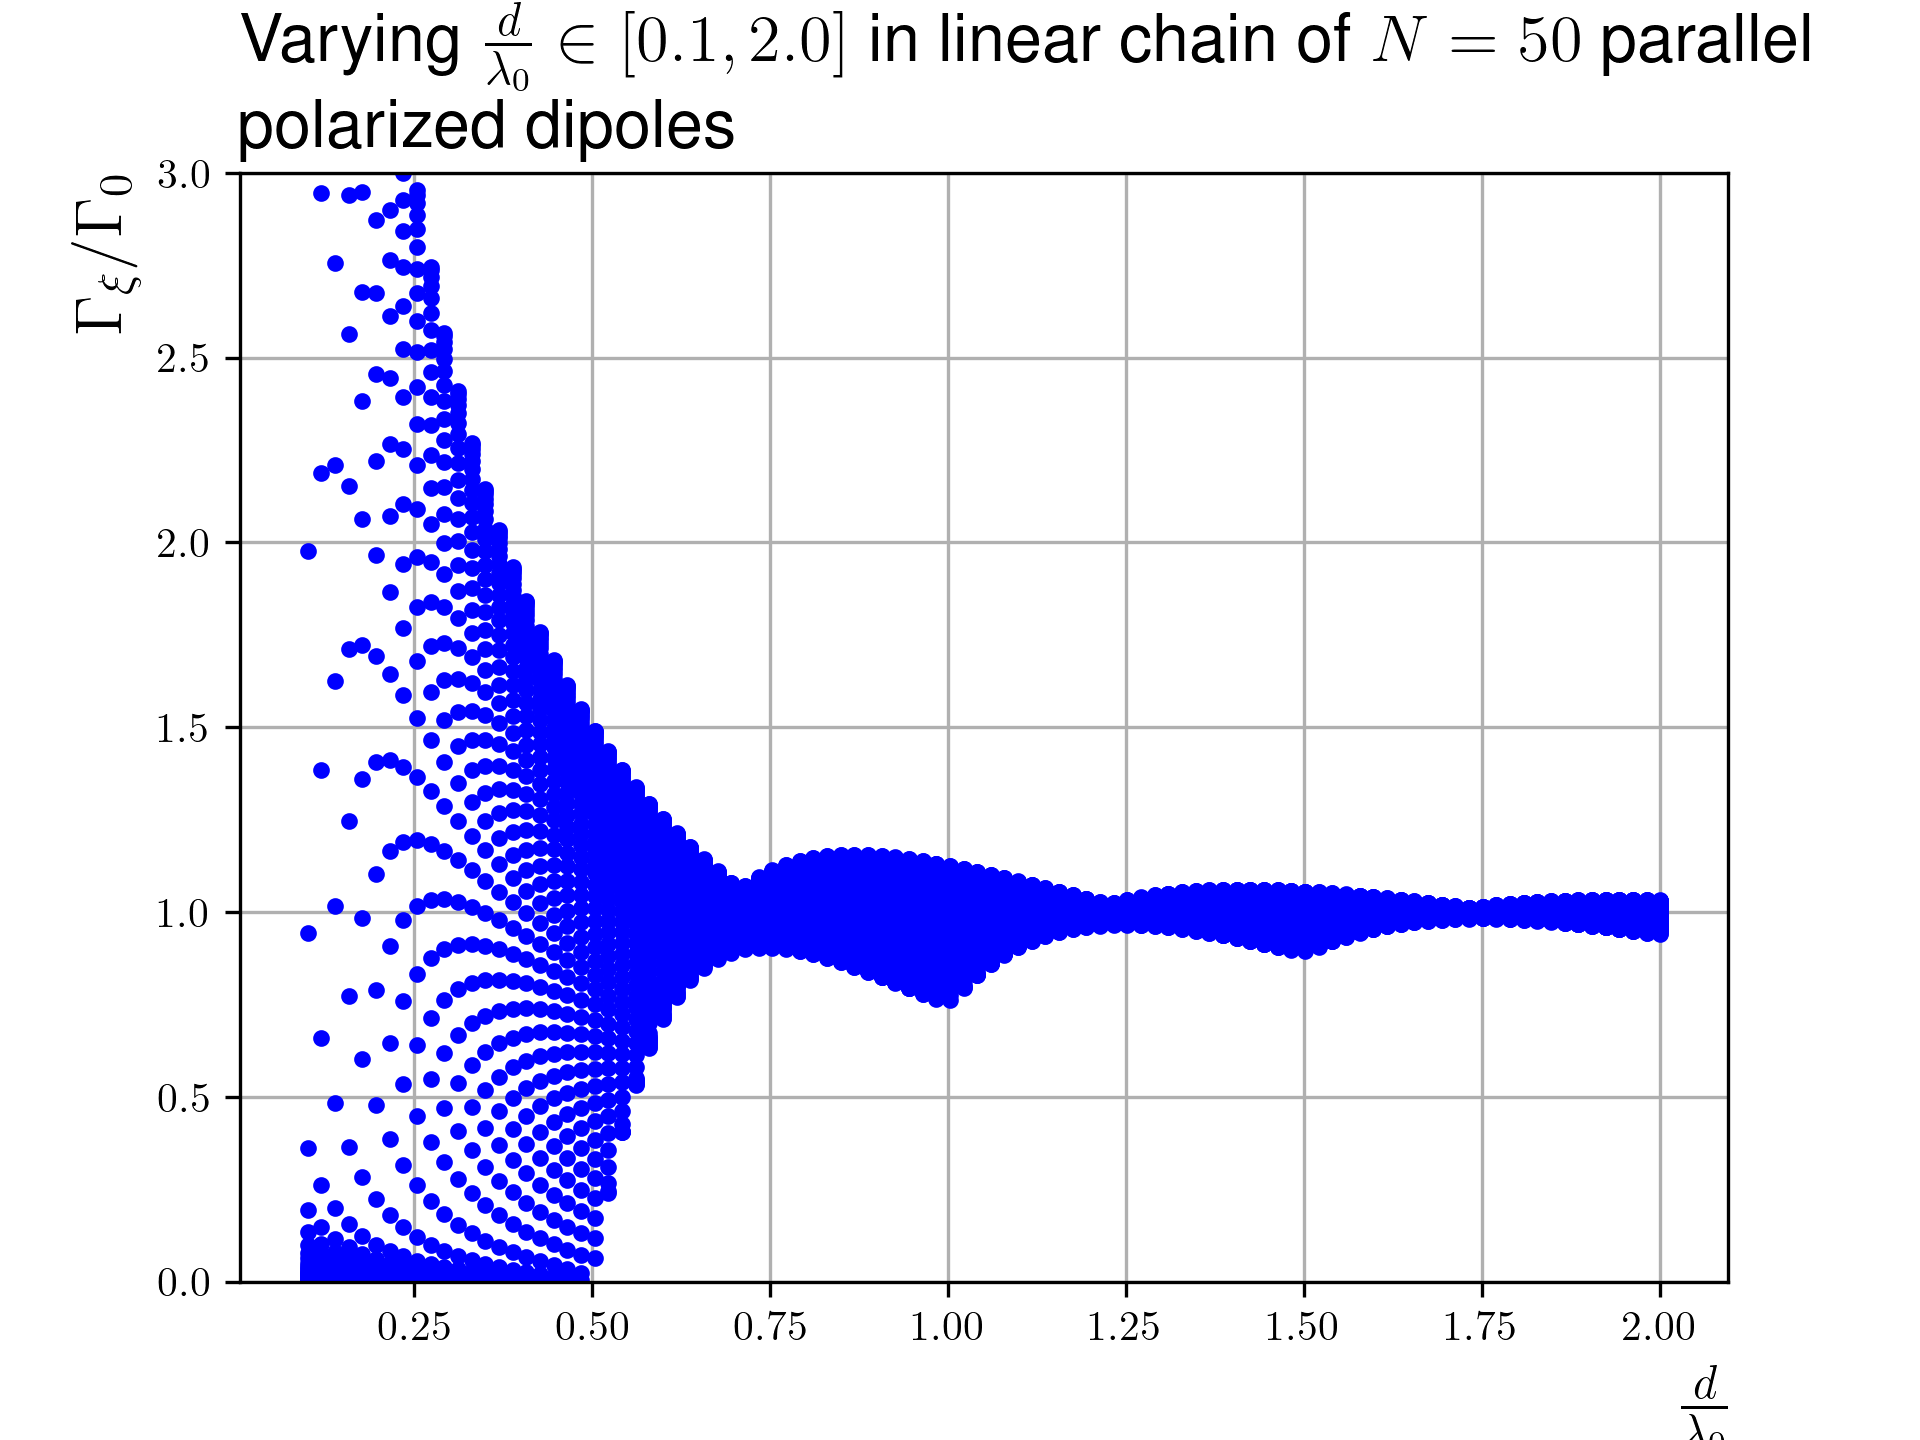
\includegraphics[width=\textwidth]{figs/case_linear_parallel_var_distance_01_2.png}
        \caption{}
        \label{fig:linear_chain_decayrates_distance_N50}
    \end{subfigure}
    \hfill
    %Figure top right corner
    \begin{subfigure}[b]{0.49\textwidth}
        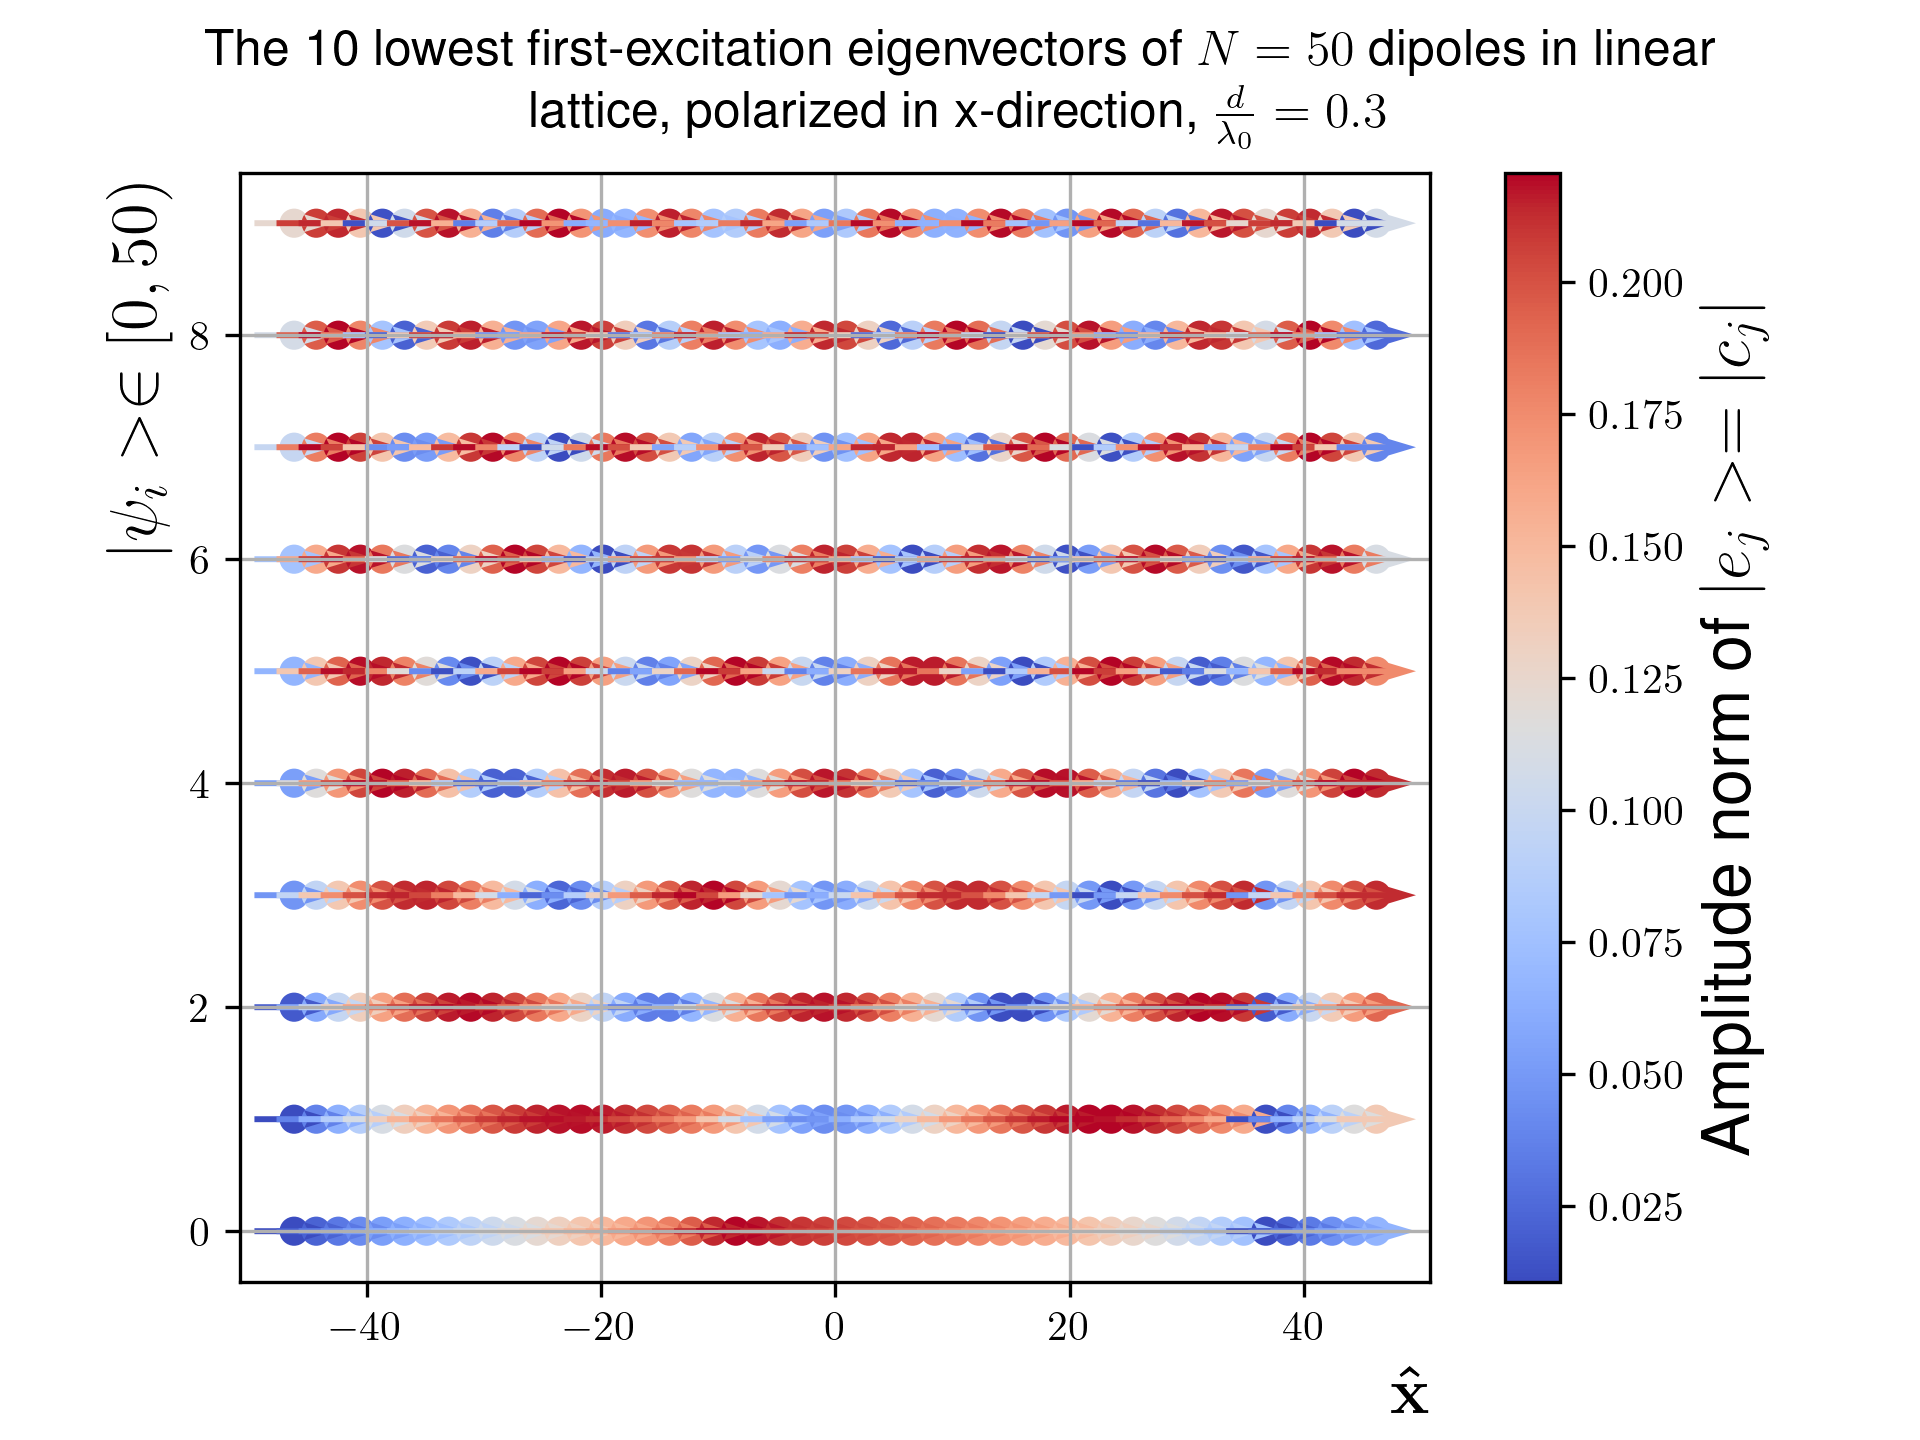
\includegraphics[width=\textwidth]{figs/dipoles_case_linear_parallel_10loweststates.png}
        \caption{}
        \label{fig:linear_chain_10loweststates}
    \end{subfigure}

    %Bottom left corner
    \begin{subfigure}{0.49\textwidth}
        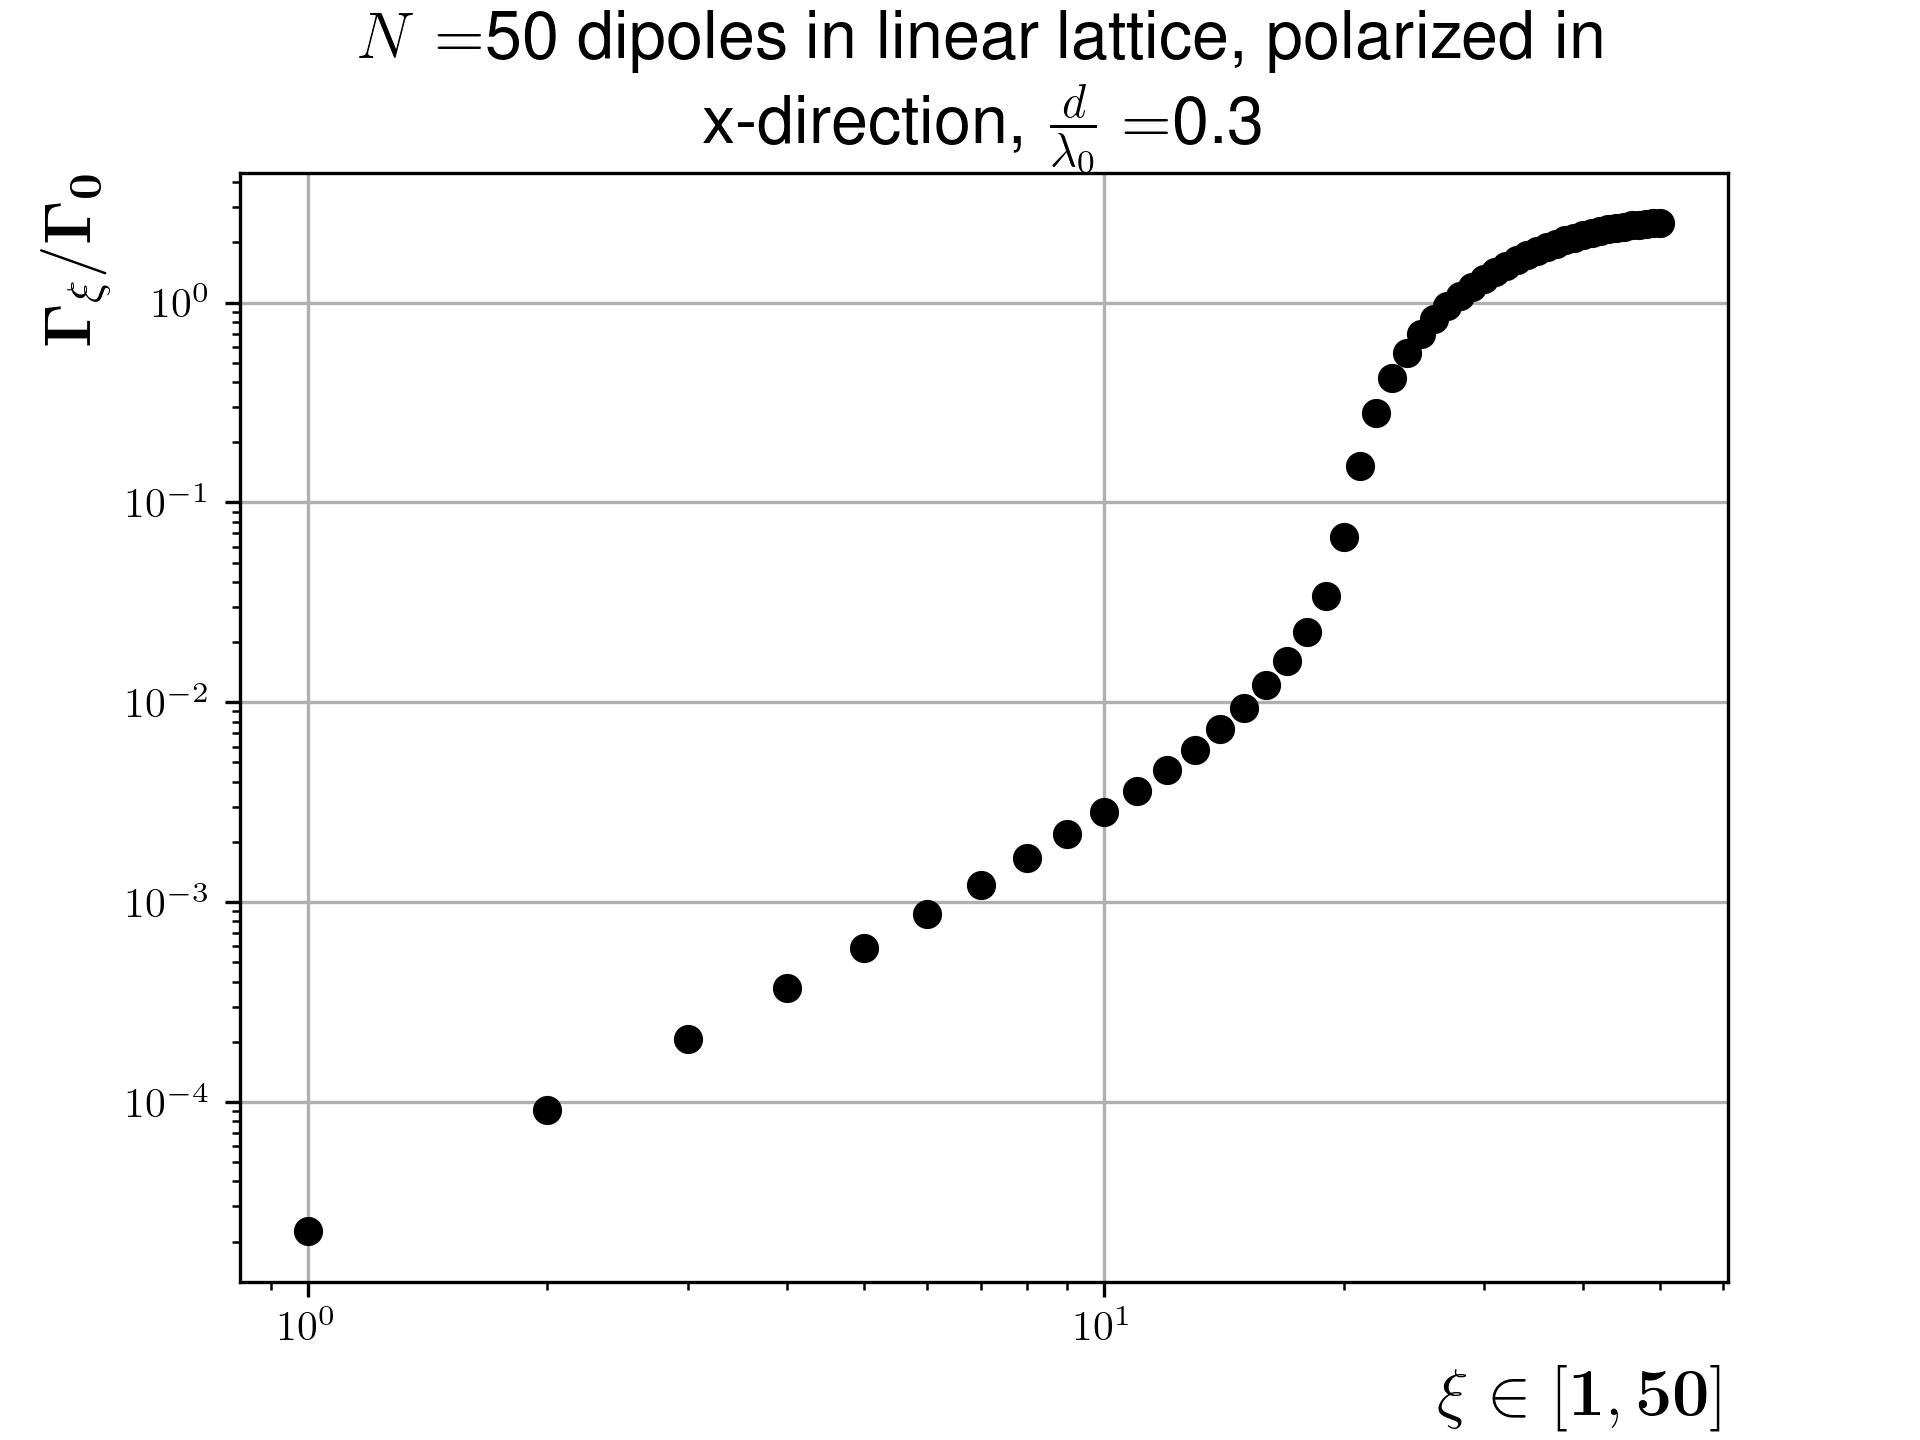
\includegraphics[width=\textwidth]{figs/case_linear_parallel_d_03.png}
        \caption{}
        \label{fig:linear_chain_decayrates}
    \end{subfigure}
    \hfill
    %Bottom right corner
    \begin{subfigure}{0.49\textwidth}
        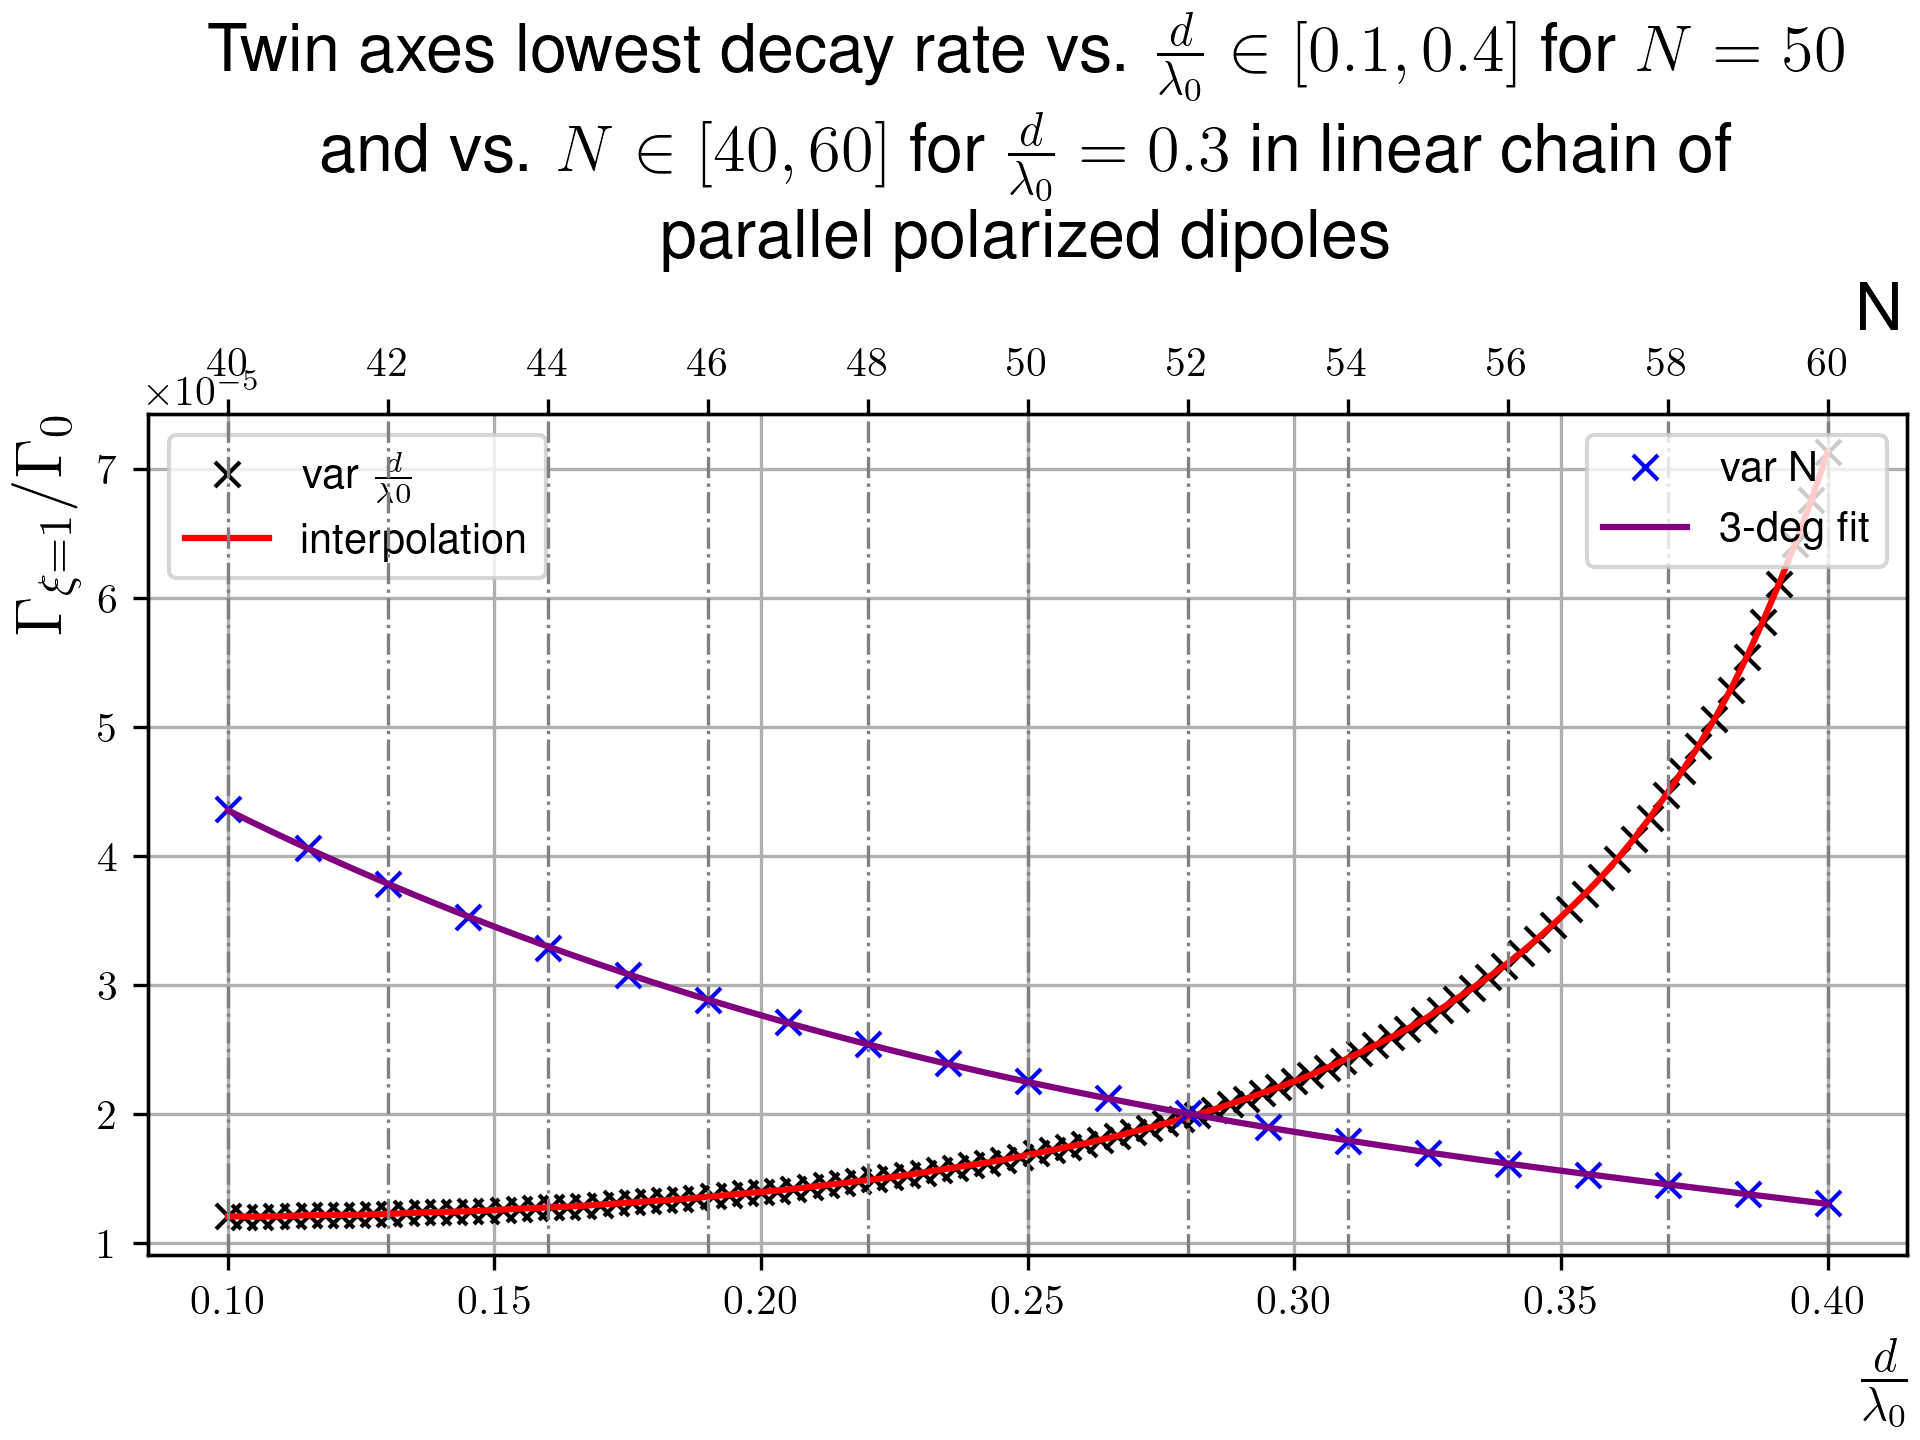
\includegraphics[width=\textwidth]{figs/case_linear_parallel_var_distance_01_04_var_N_40_60_lowest.png}
        \caption{}
        \label{fig:linear_chain_decayrates_var_dist_N}
    \end{subfigure}
    \caption{Note: chain and lattice is used interchangably, but refer in this case to the same thing: a linear one-dimensional lattice. a) Decay rates of $N=50$ linear chain with dipole moments aligned in parallel to the chain. Each vertical line of points represent the decay rates of the 50 eigenstates at the given distance. Similar tendencies as Figure 3a of (REF Asenjo). b) The 10 lowest decay rate eigenvectors visualized by the norm of the amplitudes, $\| c_j \|$, on each basisvector, i.e. $\ket{\psi_\xi} = \sum_{j=1}^N c_j \ket{e_j}$. Lattice constant: $\frac{d}{\lambda_0} = 0.3$. c) With the same lattice constant as in b), the 50 decay rates have been ranged from lowest to greatest in a loglog plot. Note: These values corresponds to the values of the vertical line at 0.3 in a). d) The lowest decay rate of parallel polarized linear chain vs. two variables. Firstly, against lattice vector (black points) for $N=50$ with linear interpolation between each point (red line) and secondly against number of atoms in chain (blue points) for $\frac{d}{\lambda_0} = 0.3$ with a third degree fit (purple line). Note the y-axis on order of $10^{-5}$. }
    \label{fig:fig1}
\end{figure}

Based on comparison with these plots and Figure 3 of (REF Asenjo), the computation is verified (behøver jeg verificere???). In Figure \ref{fig:linear_chain_decayrates_distance_N50}, it is seen that there is no significantly subradiant modes before $\frac{d}{\lambda_0} < 0.5$, i.e. when the distance between the atoms are less than half the wave-length. This property of the system is analytically motivated, as noted in Section IIIA of (REF Asenjo), since the lattice vector must be $d < \frac{\lambda_0}{2}$ to support guided modes in the infinite linear chain. This will serve as a guideline for choosing lattice constants in the following cases. In Figure \ref{fig:linear_chain_10loweststates}, the population of the most subradiant states hints at a certain structure. With some resemblance to the well-known particle in a 1D square well, the populations seem to agree with the Ansatz of (REF Asenjo, Section IIIB) for single-excitation modes in a linear chain, which states for probability amplitude of site j, of mode with wavewector $k_\xi$: 
\begin{equation}\label{eq:ansatz}
    \begin{split}
        & c^j_{ans,k_\xi} = \sqrt{\frac{2}{N + 1}} cos(k_\xi x_j), if \xi odd \\
        & c^j_{ans,k_\xi} = \sqrt{\frac{2}{N + 1}} sin(k_\xi x_j), if \xi even \\
        & k_\xi d = \frac{\pi \xi}{N + 1}
    \end{split}
\end{equation}
Where d is the interatomic distance, and $\xi$ labels the N modes. These "ansatz-states" are used as a benchmark for the computed states and respective decay rates. In particular, the overlap of the wavefunctions are computed, and the expected decay-rates for the "ansatz-states" are determined by the expectation value of the effective Hamiltonian and plotted together with the computed decay rates in Figure \ref{fig:linear_chain_decayrates}:
\begin{equation}\label{eq:overlap}
    \begin{split}
        &\mathscr{F}_{ans,\xi} = |\bra{\psi_{ans,\xi}}\ket{\psi_\xi}|^2 \\
        &\frac{\Gamma_{ans,\xi}}{\Gamma_0} = -2 Im \left( \bra{\psi_{ans,\xi}} \hat{H}_{eff} \ket{\psi_{ans,\xi}} \right)
    \end{split}
\end{equation}

TODO: Compute overlap in wavefunctions (HOW TO VISUALIZE?) , Compute decay rates og plot i Figur 1C. Finally, in Figure \ref{fig:linear_chain_decayrates_var_dist_N}, the most subradiant state's decay rate is plotted against varying the interatomic distance and number of atoms. For the case of varying distance (black and red interpolation), the number of atoms is static at $N=50$. For the case of varying number of atoms (blue and purple fit), the distance is static at $\frac{d}{\lambda_0} = 0.3$. As brought in (REF Zhang \& Mølmer), the most subradiant mode's decay rate dependency of an infinite linear chain is found to be cubic in N: $\Gamma_{\xi=1} \propto N^{-3}$, which aligns well with the cubic fit ( det er jo hyperbel fit vi skal bruge!). Regarding the varying distance, Section \ref{sec:N2} sheds some light, albeit not for many N, on the decay rate dependency of distance. It is seen that the Green's function's leading term for small distances is a $\frac{1}{r^3}$-term, also for the imaginary parts, which ends up determining the decay rate. However, for small distances we also have $sin(r) \approx r$, so the leading term for imaginary parts will be $\frac{1}{r^2}$. This may explain the change in curvature, which is noticable for the red interpolation line that resembles an exponential function. It cannot be exponential, as evidently in Figure \ref{fig:linear_chain_decayrates_distance_N50}. Distances greater than $\frac{d}{\lambda_0} = 0.5$ has the decay rate oscillating around 1, and for distances even greater, the interaction between the dipoles weaken, leaving the atoms with the the vacuum spontaneous emission rate. 

Since the modes with a wavevector within the first Brillouin zone are guided modes (REF Asenjo), the only permitted places for the system to emit photons are at the ends of the chain. Therefore, it is hypothesized that the probability amplitude is decreased primarily, when the waves reach the end of the chain. (Men jeg undersøger jo ikke dette?)

God forklaring af figur, der viser a, b, c og d. a: decay rate rangeret, b: most subradiant mode probability amplitude, c: decay rate as function of d og endelig d: as function of N. Xi indexes the modes by decay rates from smallest to greatest. 

\subsubsection{Varying polarization in linear chain}\label{disc:linear_chain_varypola}

Vi ser også i Asenjo IIIA figur 1, at der forventes en mærkeligere opførsel for nogle tilstande, når polarisering er transversal. Måske noget der kan forklare opførslen af de superradiante tilstande. TEORI???

For the linear chain, varying the polarization does not affect the most subradiant modes' decay rates significantly. However, some change in behaviour among the superradiant modes emerged, while doing this analysis. Superradiant modes for some angles relative to the chain axis are seen in Figure \ref{fig:linear_var_angle}:
\begin{figure}[H]
    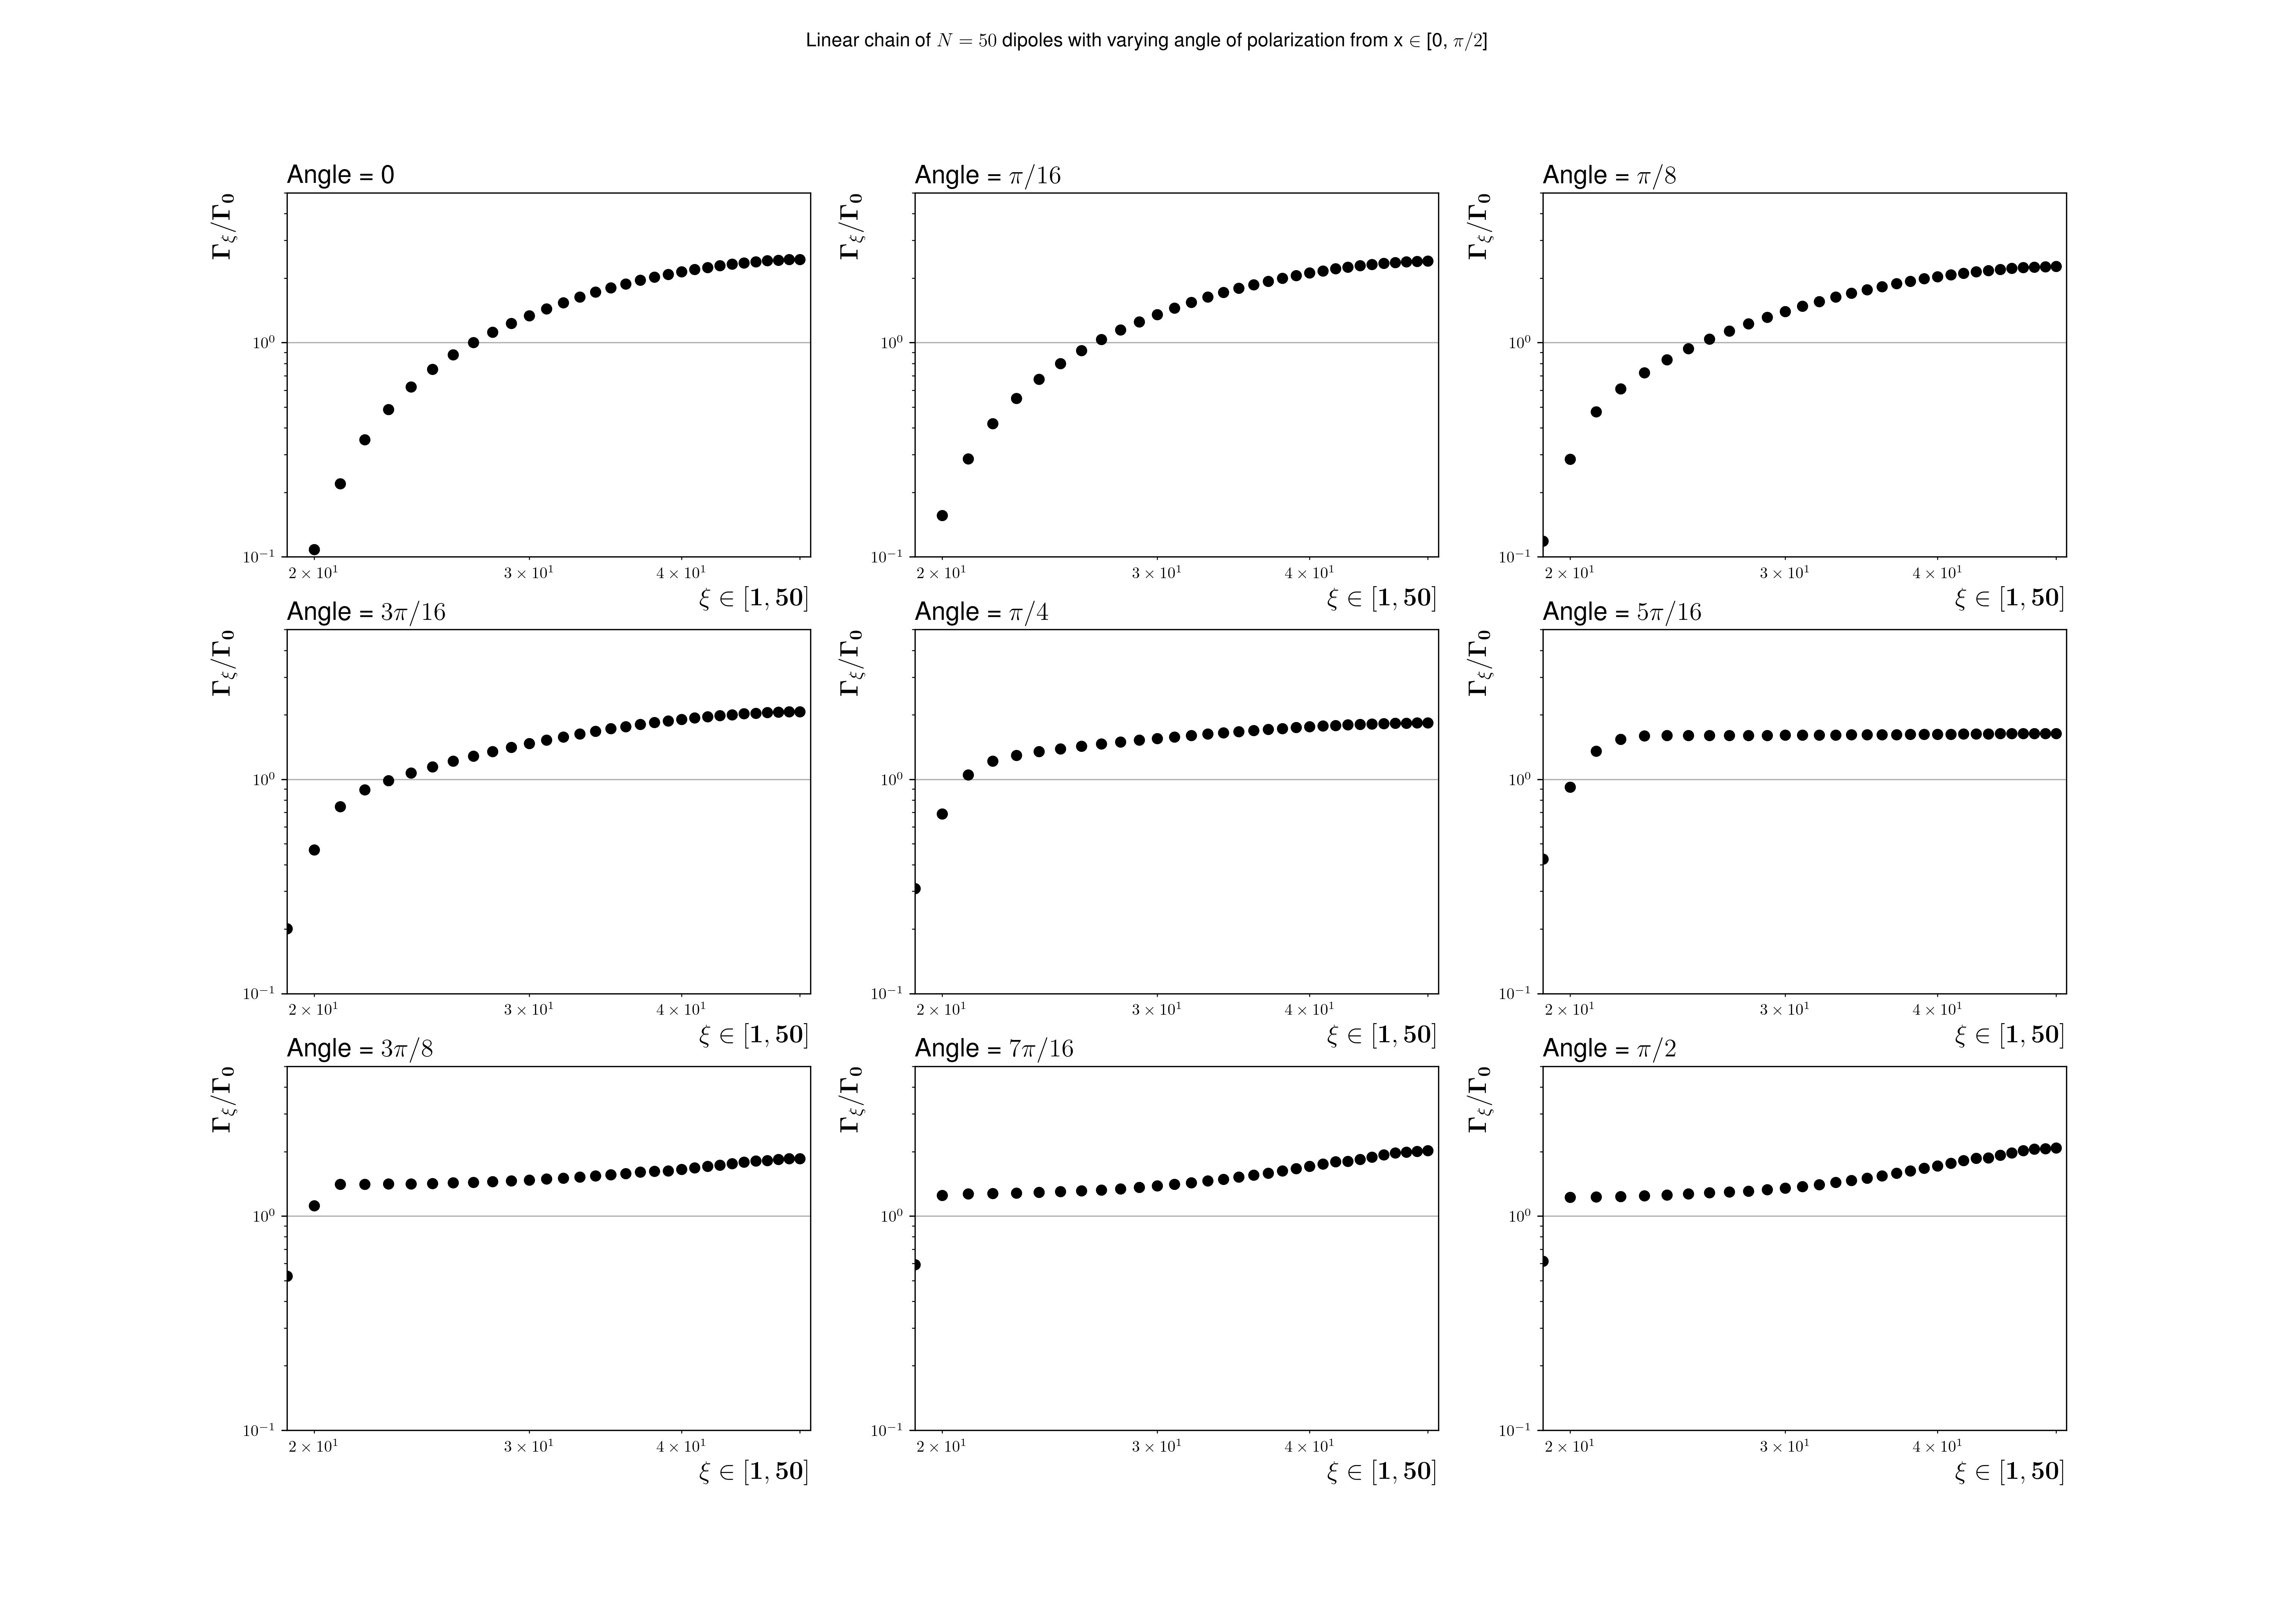
\includegraphics[width=0.99\textwidth]{figs/case_linear_var_angle_0_pi05.png}
    \caption{Varying polarization angle from parallel to perpendicular (w.r.t. chain axis), $\hat{n} = \hat{e}_x \rightarrow \hat{e}_z$, in 9 steps. The angle is given with respect to $\hat{e}_x$. The visible data points on the plots are limited to $\xi \in [20, 50]$ to give a better view of superradiant states, which seem to be affected the most by this variation. Computed with $\frac{d}{\lambda0} = 0.3$. }
    \label{fig:linear_var_angle}
\end{figure}
Above $\frac{\pi}{4}$, the superradiant spectrum seems to flatten out, and then slightly increase again towards the perpendicular polarization. How the constructive / destructive intererference varies with polarization is a difficult question to answer for many dipoles. As seen in Section \ref{sec:N2}, an expression for this dependency is given in the $N=2$ case, which suggests a WHAT relation. This...

\subsubsection{Broken chain}\label{disc:linear_broken}

In Figure \ref{fig:linear_broken}, the linear chain is "broken" on the middle with varying angle, and the population of $\ket{\psi_{\xi=1}}$ is visualized with a colorbar. Note: the probabilites in this case do not add up to 1. From top to bottom: $p_{total} = [0.95, 0.88, 0.89]$. As discussed in Section \ref{sec:full_system}, this is incorrect in Quantum Mechanics, but remember, the Hamiltonian in question is in fact not Hermitian, which removes the guarantee of a completely orthonormal basis. If the probabilites do not add up to one, the eigenvectors are not normalized. As also noted, the missing probability is attributed to the atoms becoming deexcited and exciting a photon mode. In that picture, this suggests that even the most subradiant modes in a broken chain have a significant probability of instantaneously emitting a photon. 
\begin{figure}[H]
    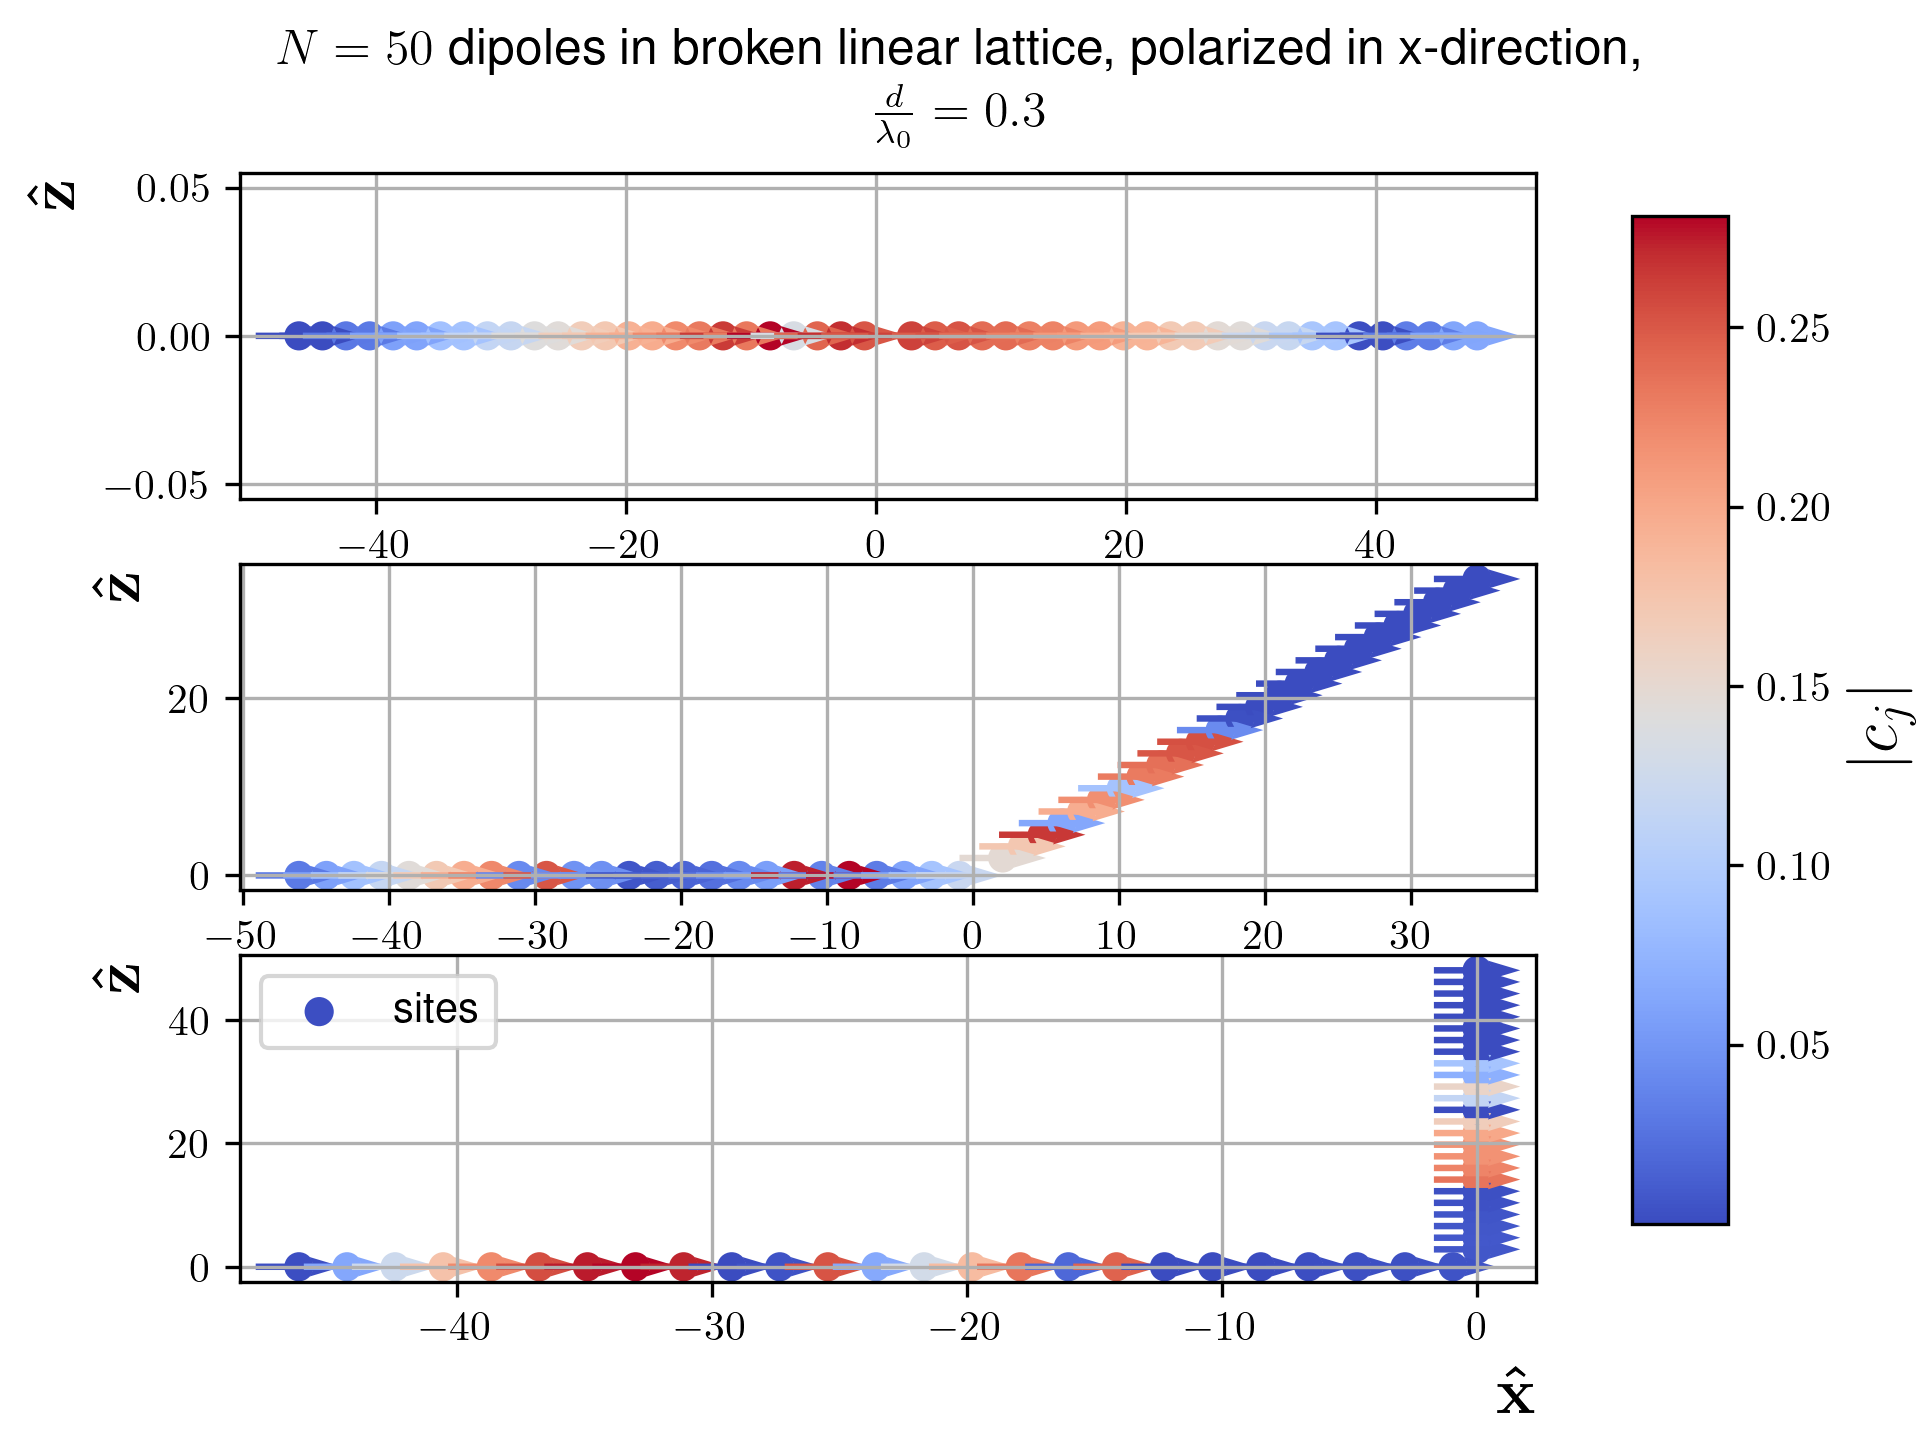
\includegraphics[width=0.9\textwidth]{figs/dipoles_case_linear_broken.png}
    \caption{Three cases of a broken linear lattice with angles $\{0, \frac{\pi}{4}, \frac{\pi}{2}\}$ polarized along x-axis (non-broken chain axis) with $N = 50$ and $\frac{d}{\lambda_0} = 0.3$. The population on the chain of the most subradiant mode is visualized with the colorbar.}
    \label{fig:linear_broken}
\end{figure}
As expected, the population of the unbroken case is localized in the middle (with a few unexpectedly exempted sites, with a bit lower population), as it is also seen in Figure \ref{fig:linear_chain_10loweststates}. In the two broken cases however, the population is delocalized. MORE. In Figure \ref{fig:linear_broken_rates}, the decay rate of the most subradiant state is plotted against varying angle of the broken chain:
\begin{figure}[H]
    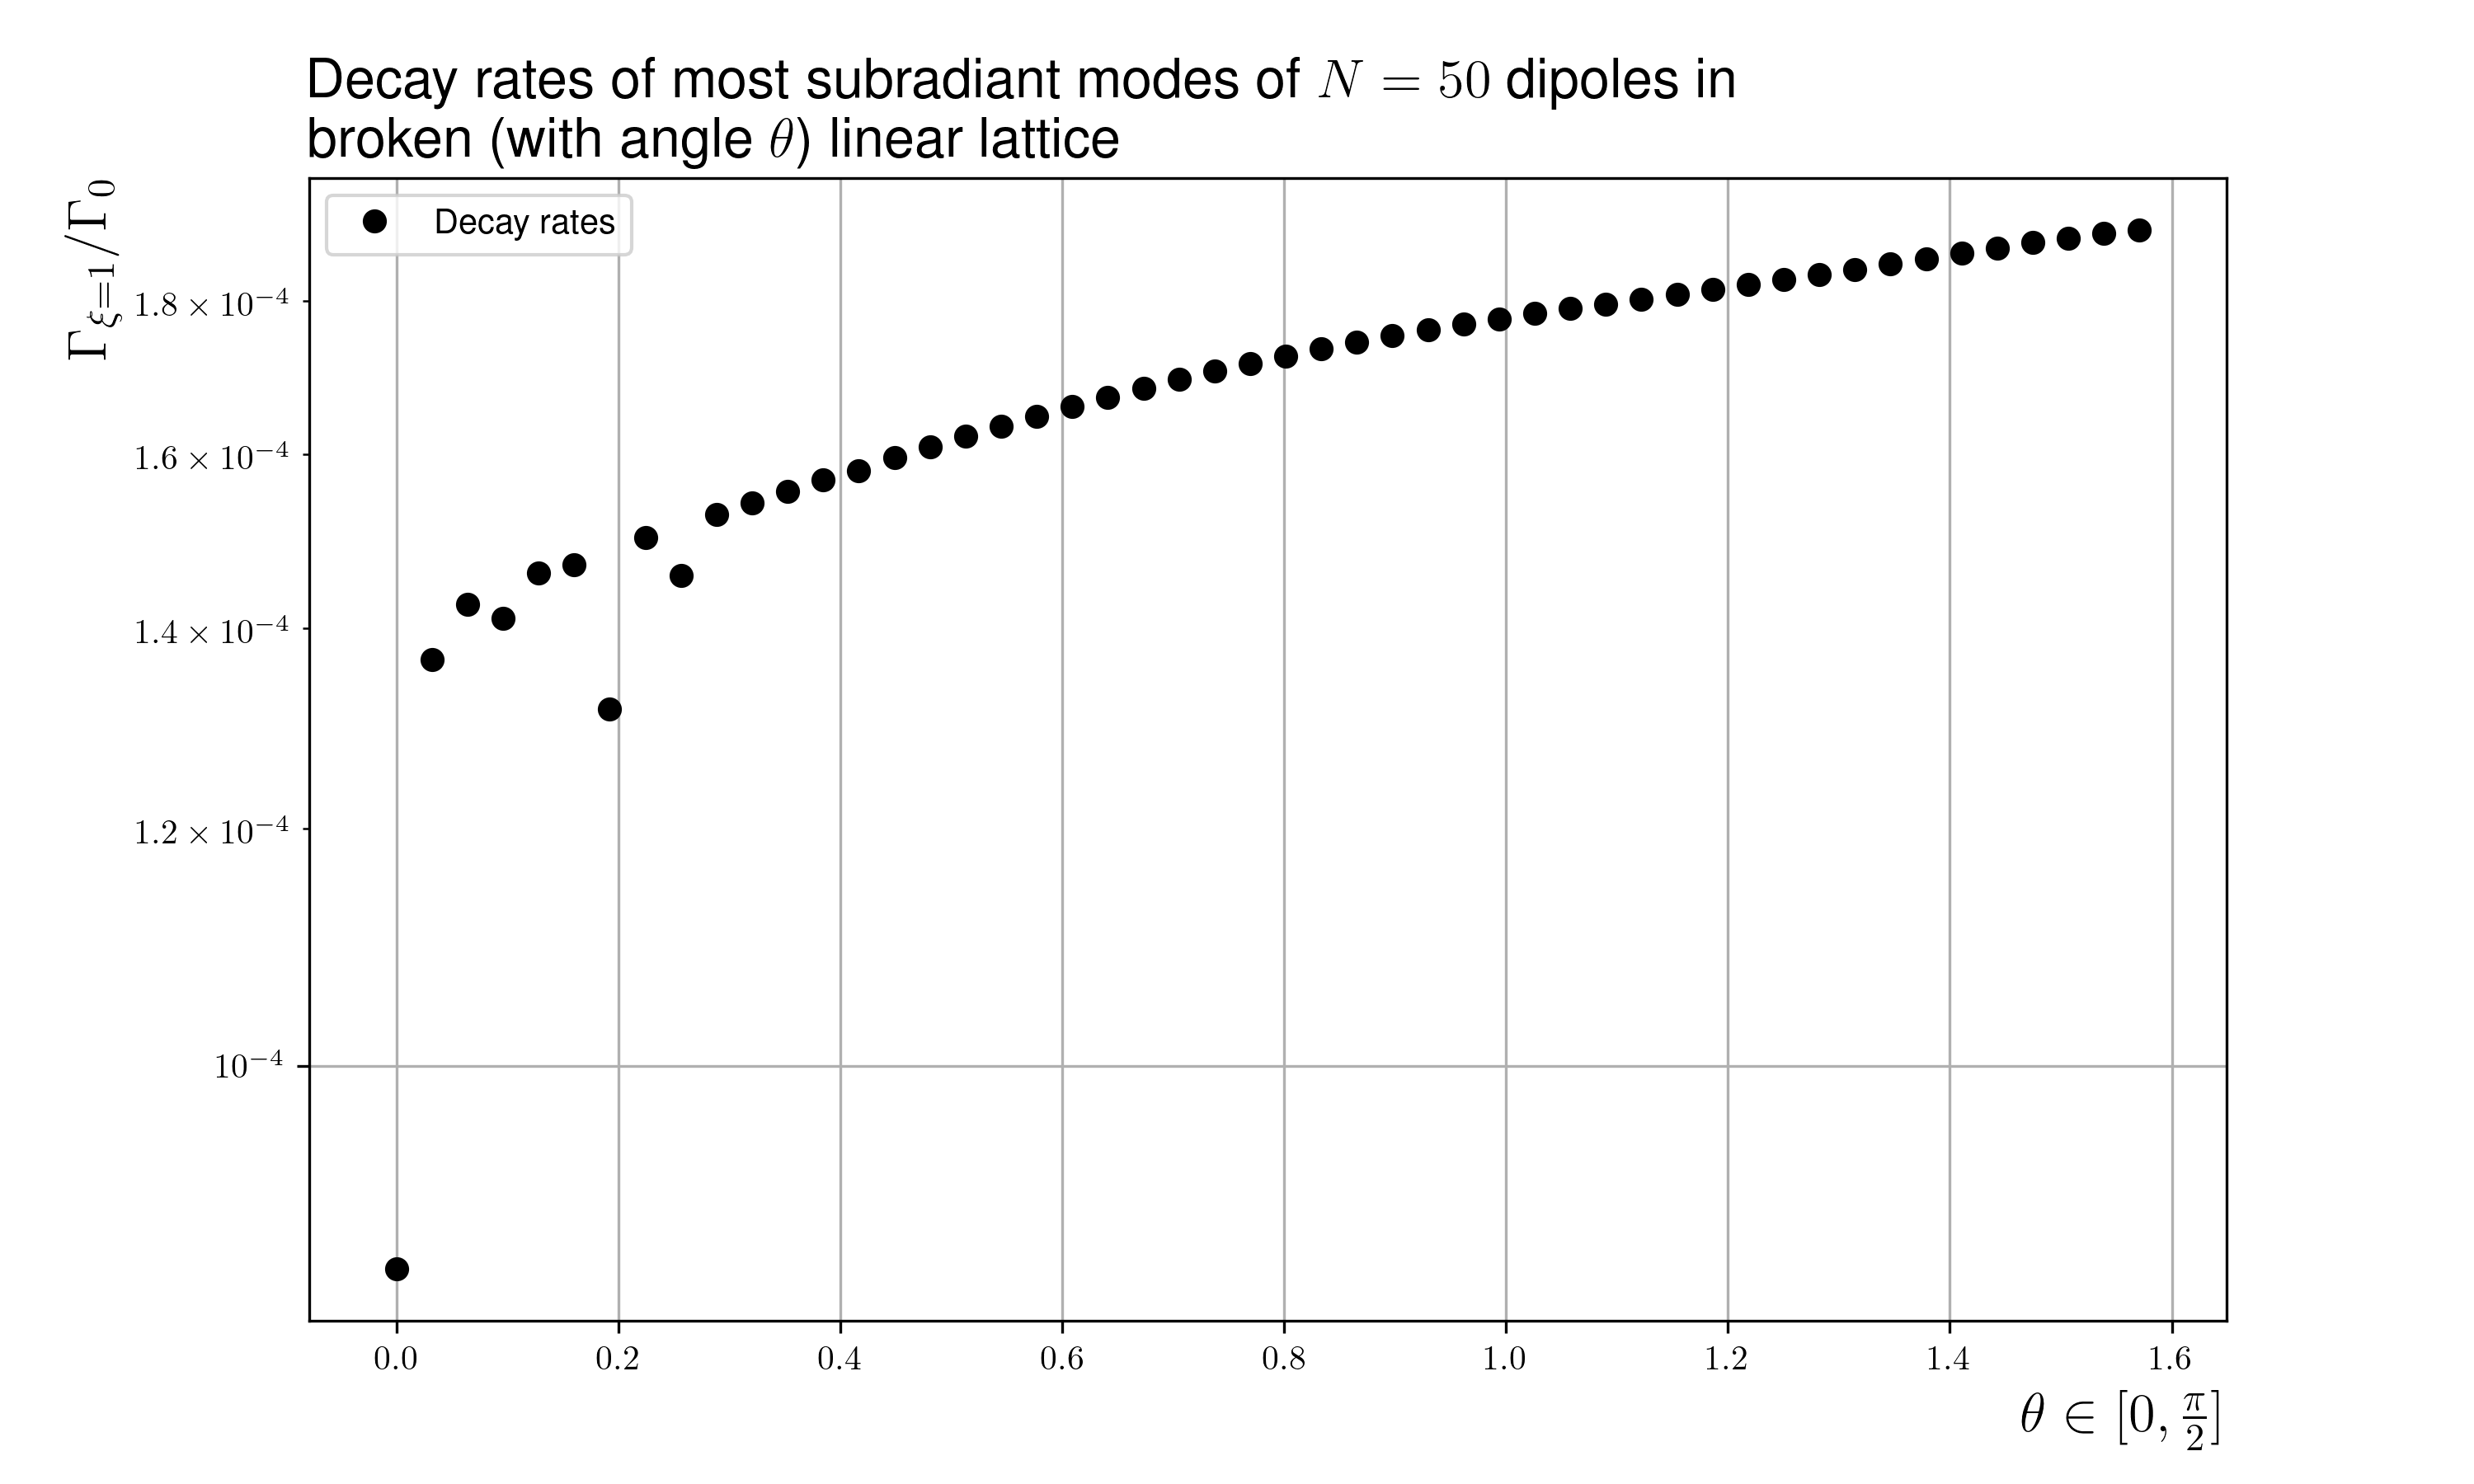
\includegraphics[width=0.9\textwidth]{figs/case_linear_broken_rates.png}
    \caption{Decay rate of most subradiant state vs. angle on broken chain. Dipole moments polarized along x-axis and $\frac{d}{\lambda_0} = 0.3$. }
    \label{fig:linear_broken_rates}
\end{figure}
Regarding the range of decay rates in this plot, they do not change much with increasing angle of the corner. As seen in Figure \ref{fig:linear_chain_decayrates_var_dist_N}, the decay rate for the unbroken linear chain is about $\Gamma_{\xi=1, unbroken} \approxeq 2 \cdot 10^{-5}$, but in this plot, it is closer to $\Gamma_{\xi=1, broken w. \theta = 0} \approxeq 8 \cdot 10^{-5}$. It should be the same, because the two lattices are in this case indistinguishable, which points to some error. Since the population on the chain in these cases are not equal either, something is wrong. 

For the increasing angle cases, the approximately steady decay rate of $\Gamma_{\xi = 1, broken w. \theta > 0} \approxeq 10^{-4}$ might suggest little to no dependence of the angle, but as soon as there is a break in the chain, the decay rate will increase drastically (one order of magnitude in this case). One explanation might be that the discontinuity effectively causes the one part to act as a lone linear chain, i.e. the remaining part of the chain is ignored. In this case, the break happens after $j=25$ (half-way), for which a decay rate of $\Gamma_{\xi=1, N=25} \approxeq N^{-3} = 25^{-3} = 6 \cdot 10^{-5}$ is expected for the smallest decay rate mode (assuming the cubic dependency in $N$, as discussed in Section \ref{disc:linear_chain}). 

In Section \ref{sec:further}, it is briefly discussed, what other analyses of this system might be interesting. 

\subsection{Circular chain}\label{disc:circular}

The circular lattice is particularly interesting, because the spin-wave modes of the chain never encounters a boundary, which in Section \ref{disc:linear_chain} is the hypothesized primary loss of excited probability amplitude. As seen in (REF Asenjo), the circular lattice's most subradiant mode achieves exponential decrease in decay rate as function of N, $\Gamma_{\xi = 1} \propto e^{-N}$, compared to the linear chain's $\Gamma_{\xi=1} \propto N^{-3}$. But, how does the decay rate change with variation of the polarization of the atoms? First, the circular lattice with most subradiant mode probability amplitude, decay rate as function of interatomic distance and as function of N. 

inter-atomic distances

\subsubsection{Polarized unidirectionally}

circular unidirectional. Easier to implement in reality with uniform magnetic field.

\begin{figure}[H]
    \centering
    \begin{subfigure}[b]{0.49\textwidth}
        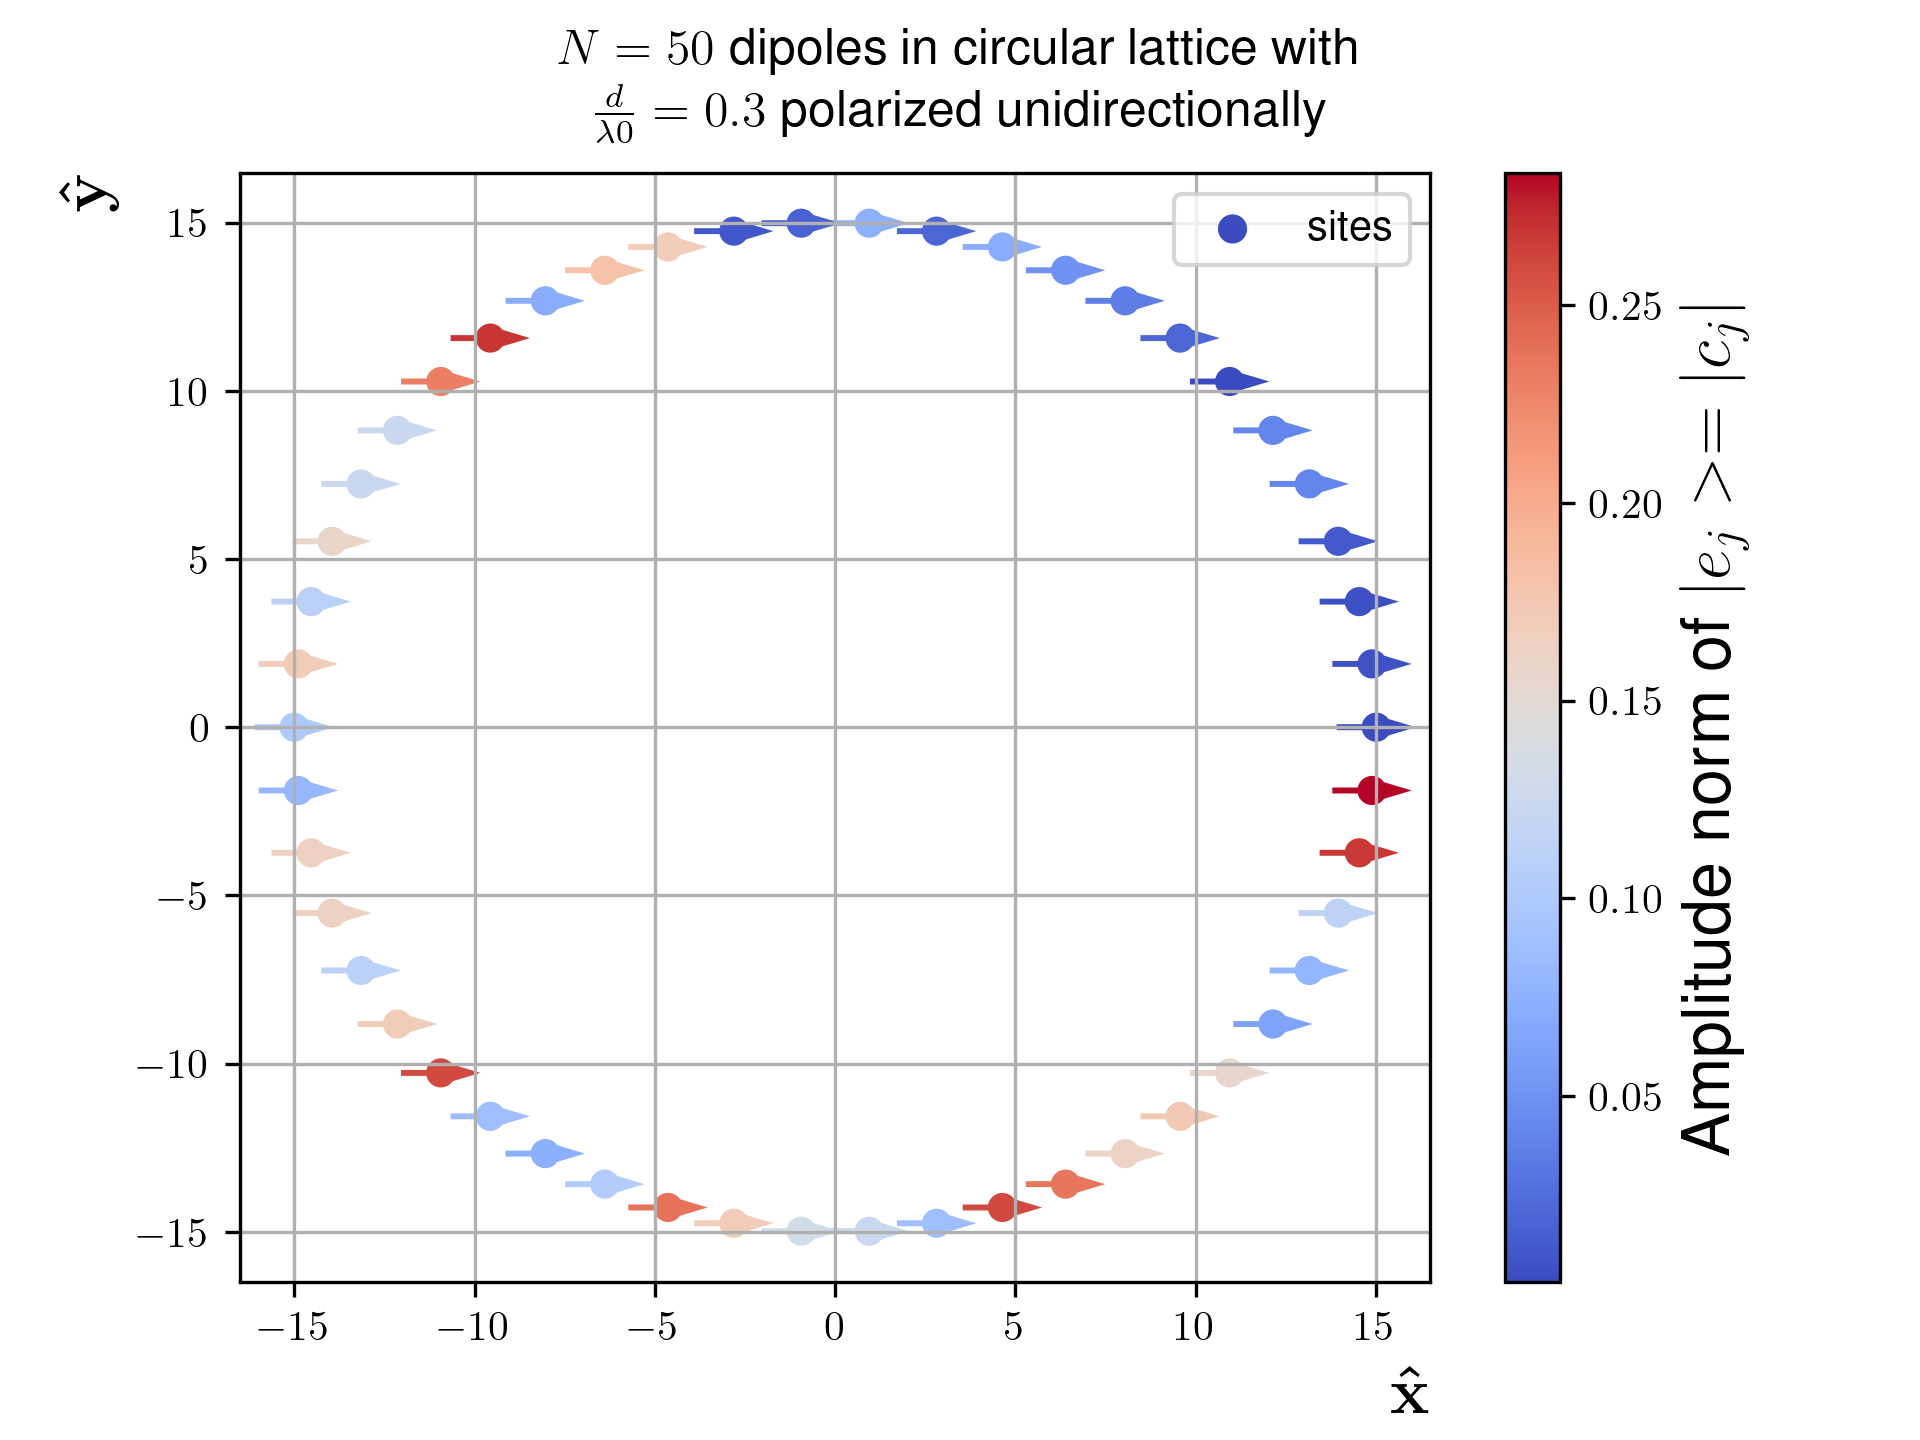
\includegraphics[width=\textwidth]{figs/dipoles_case_circular_unidirectional_lowest.png}
        \caption{}
        \label{fig:circular_lowest_eigenstate}
    \end{subfigure}
    \hfill
    \begin{subfigure}[b]{0.49\textwidth}
        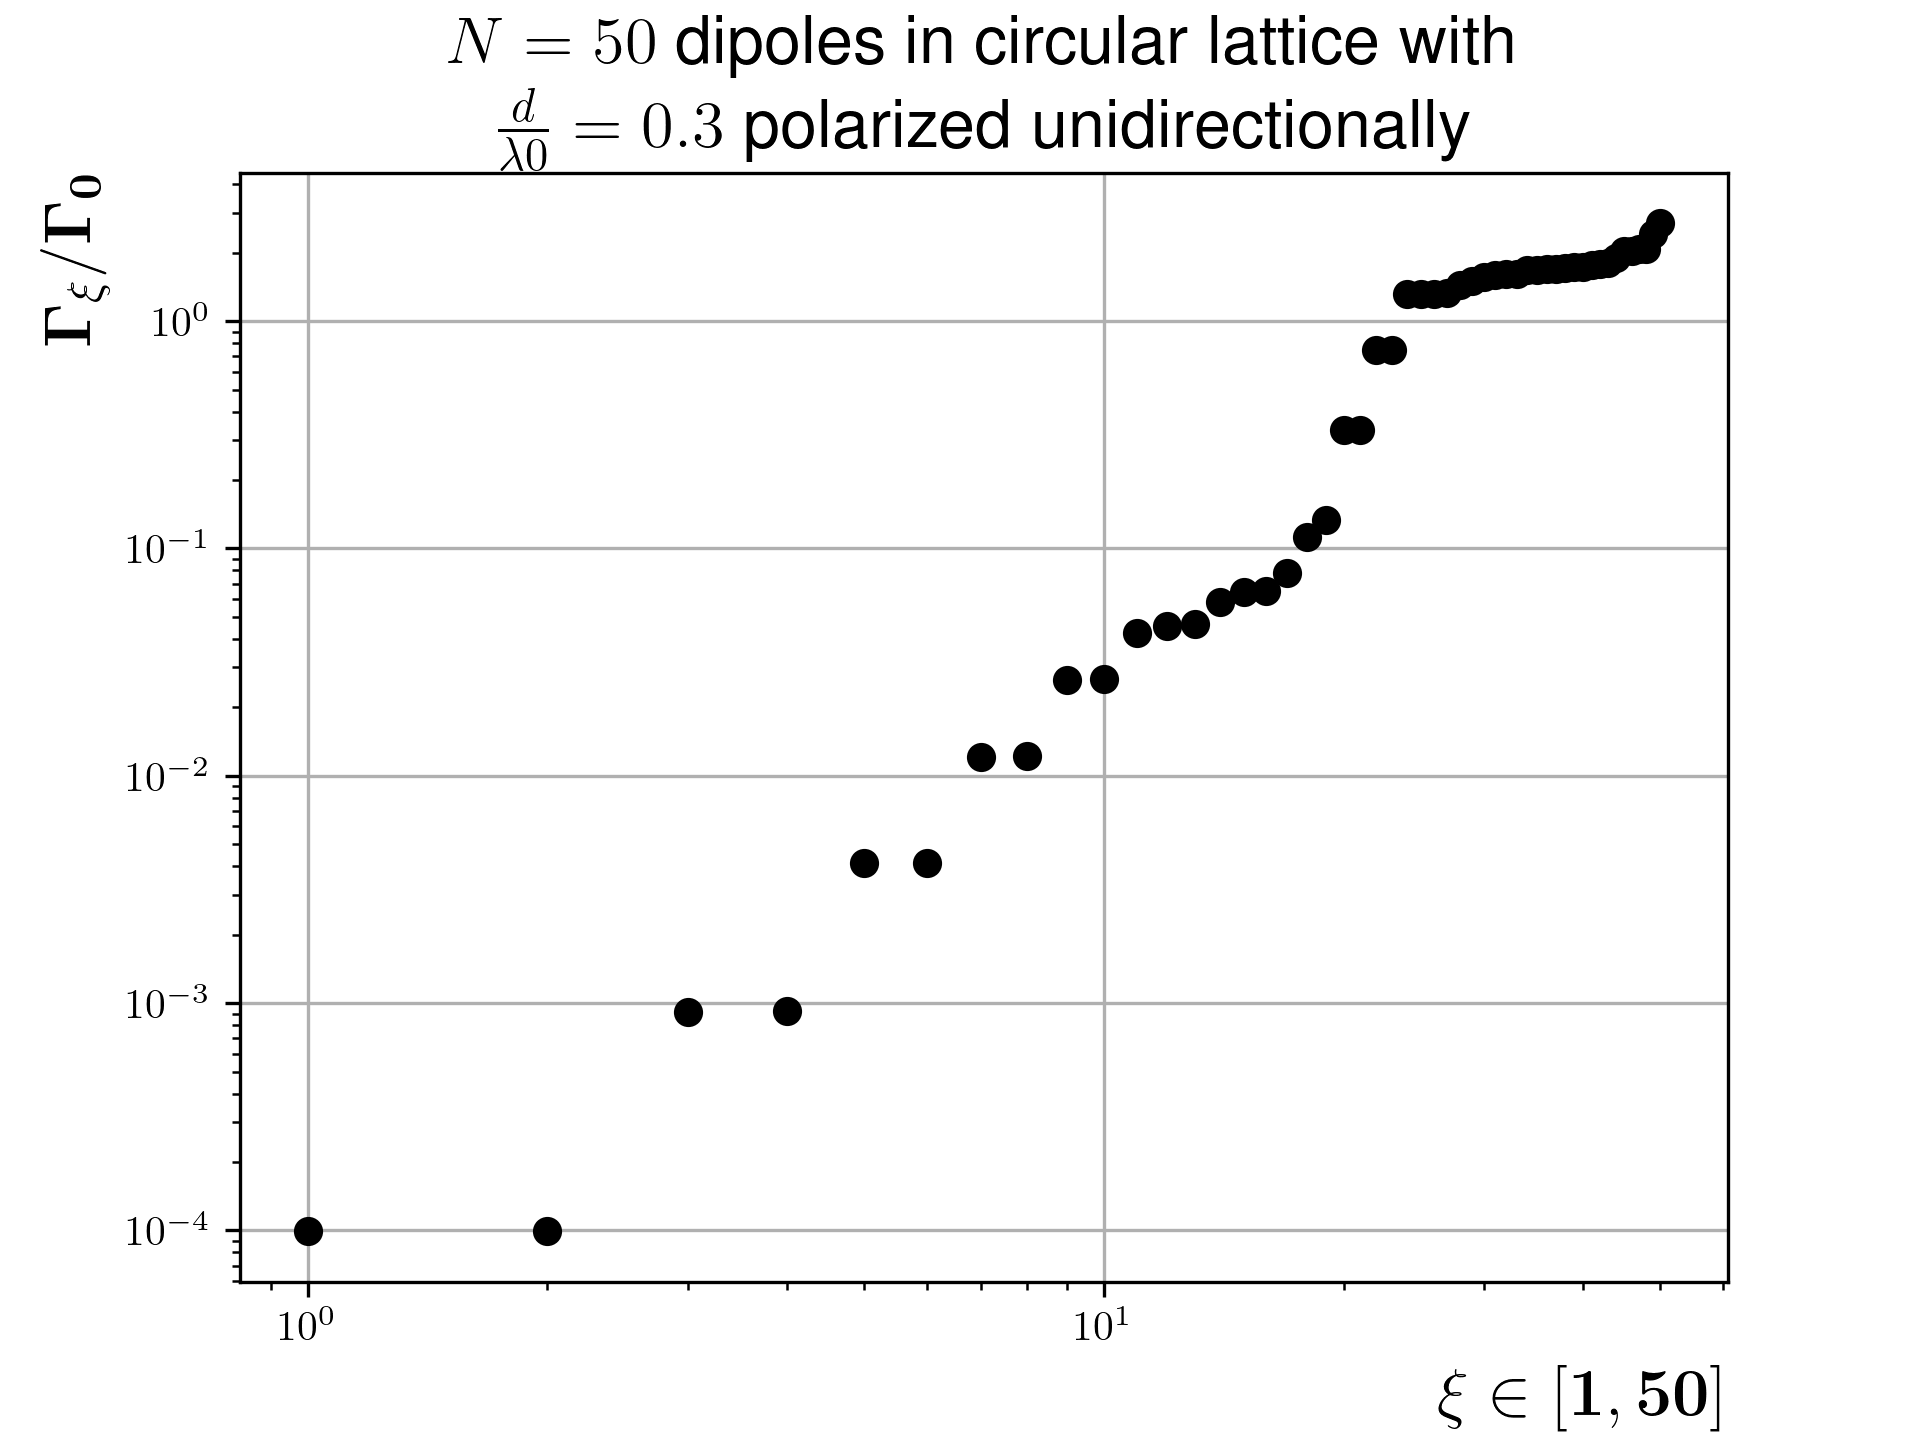
\includegraphics[width=\textwidth]{figs/case_circular_unidirectional_d_03.png}
        \caption{}
        \label{fig:circular_unidirectional_decayrates}
    \end{subfigure}
    \caption{}
    \label{fig:circular}
\end{figure}

circular varying N and d

\begin{figure}[H]
    \centering
    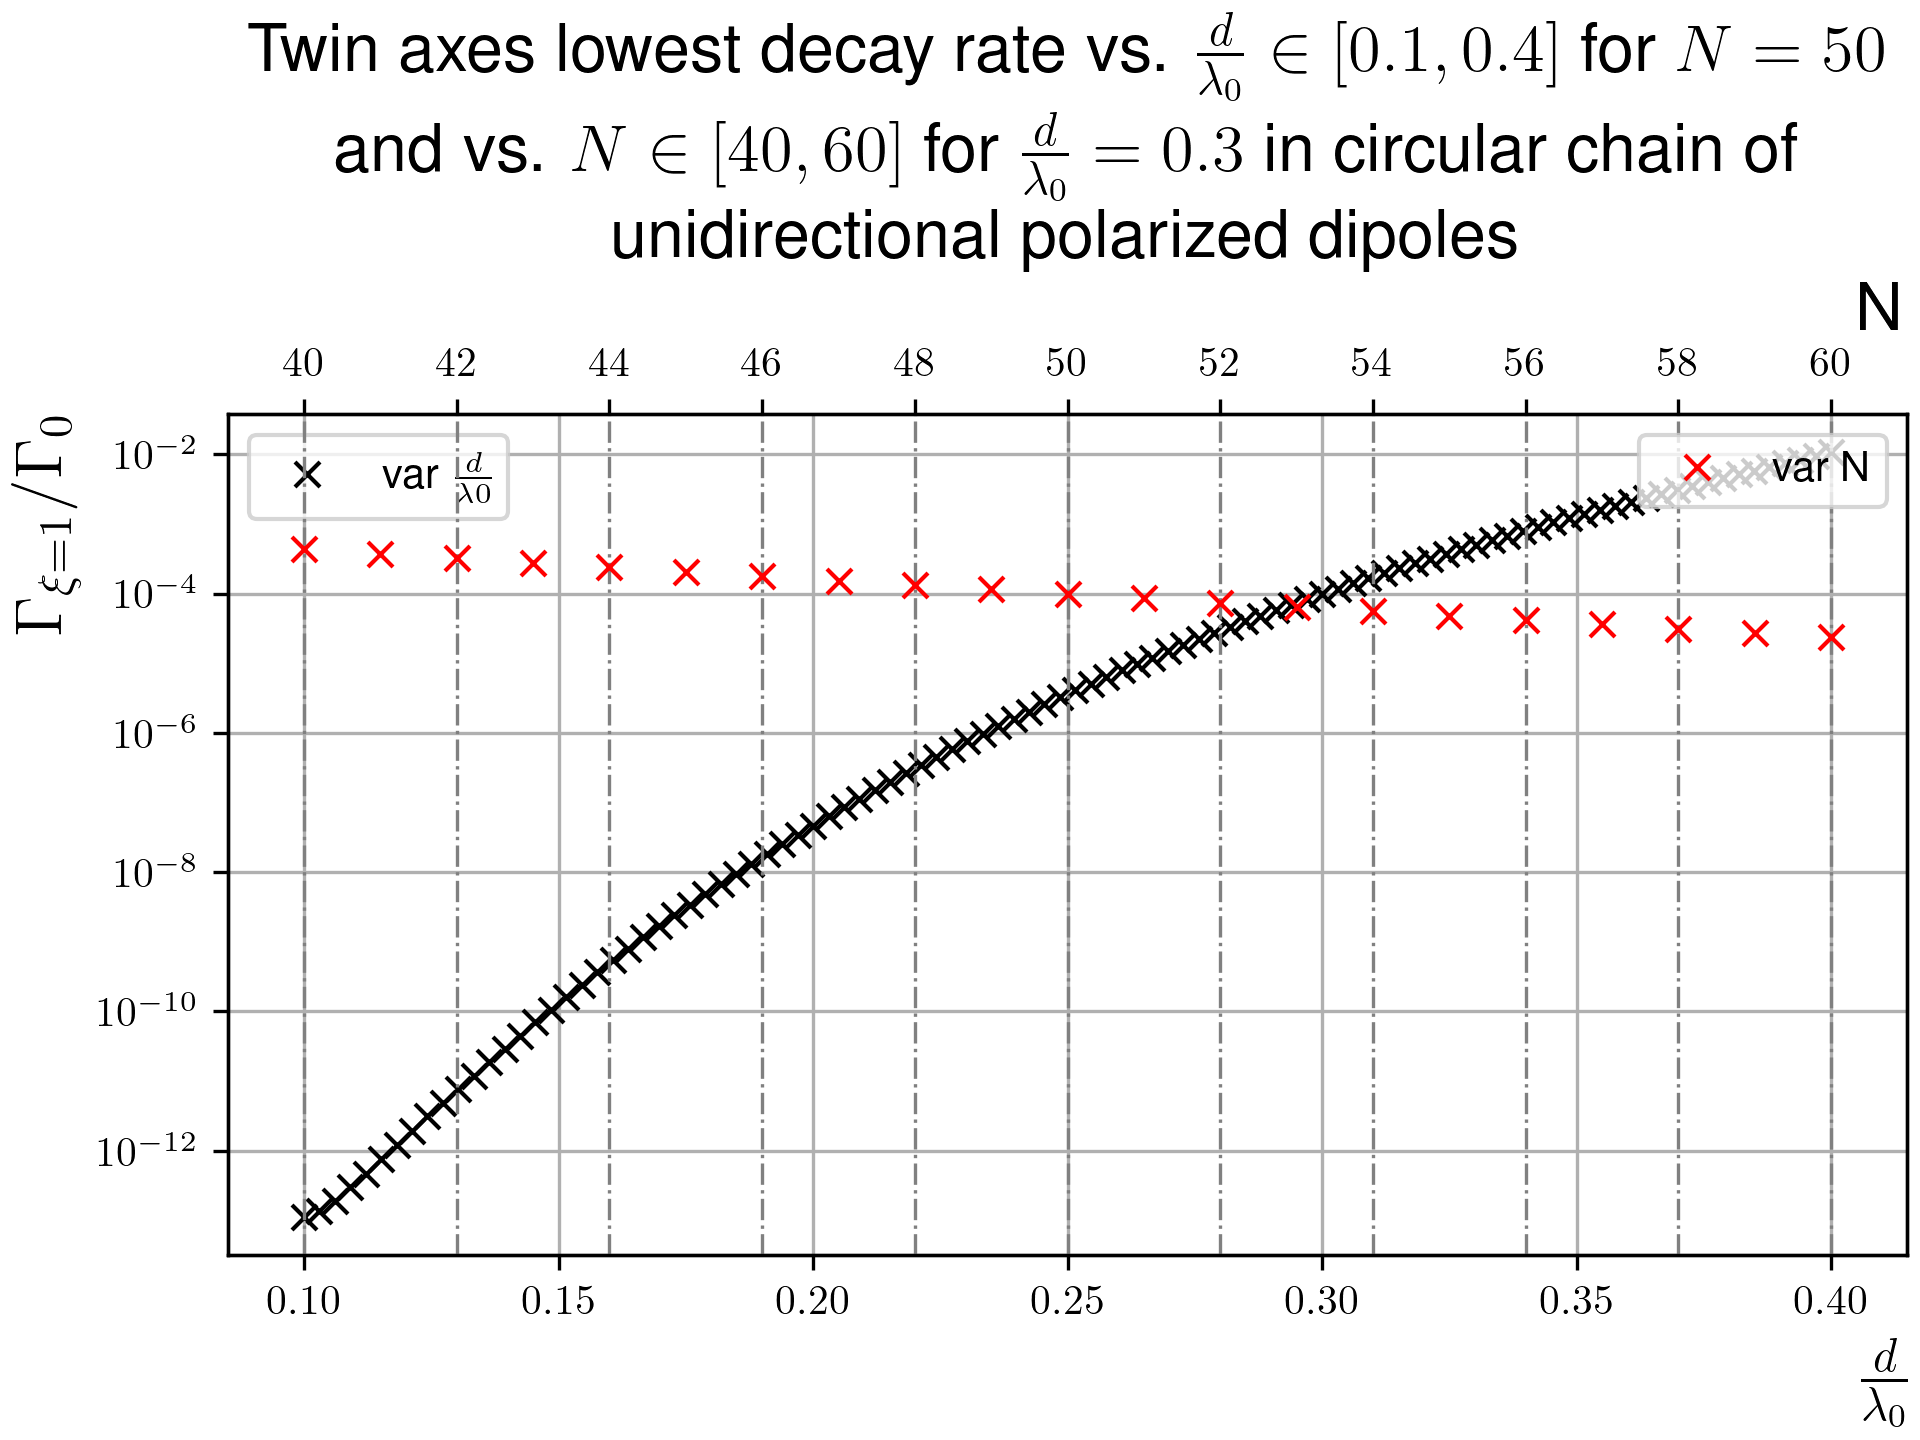
\includegraphics[width=0.9\textwidth]{figs/case_circular_unidirectional_var_distance_01_04_var_N_40_60_lowest.png}
    \caption{}
    \label{fig:circular_unidirectional_varying}
\end{figure}

\subsubsection{Polarized inwards}

circular inwards. probably a challenge to align with magnetic field (emulates magnet monopole = no-go)

\begin{figure}[H]
    \centering
    \begin{subfigure}[b]{0.49\textwidth}
        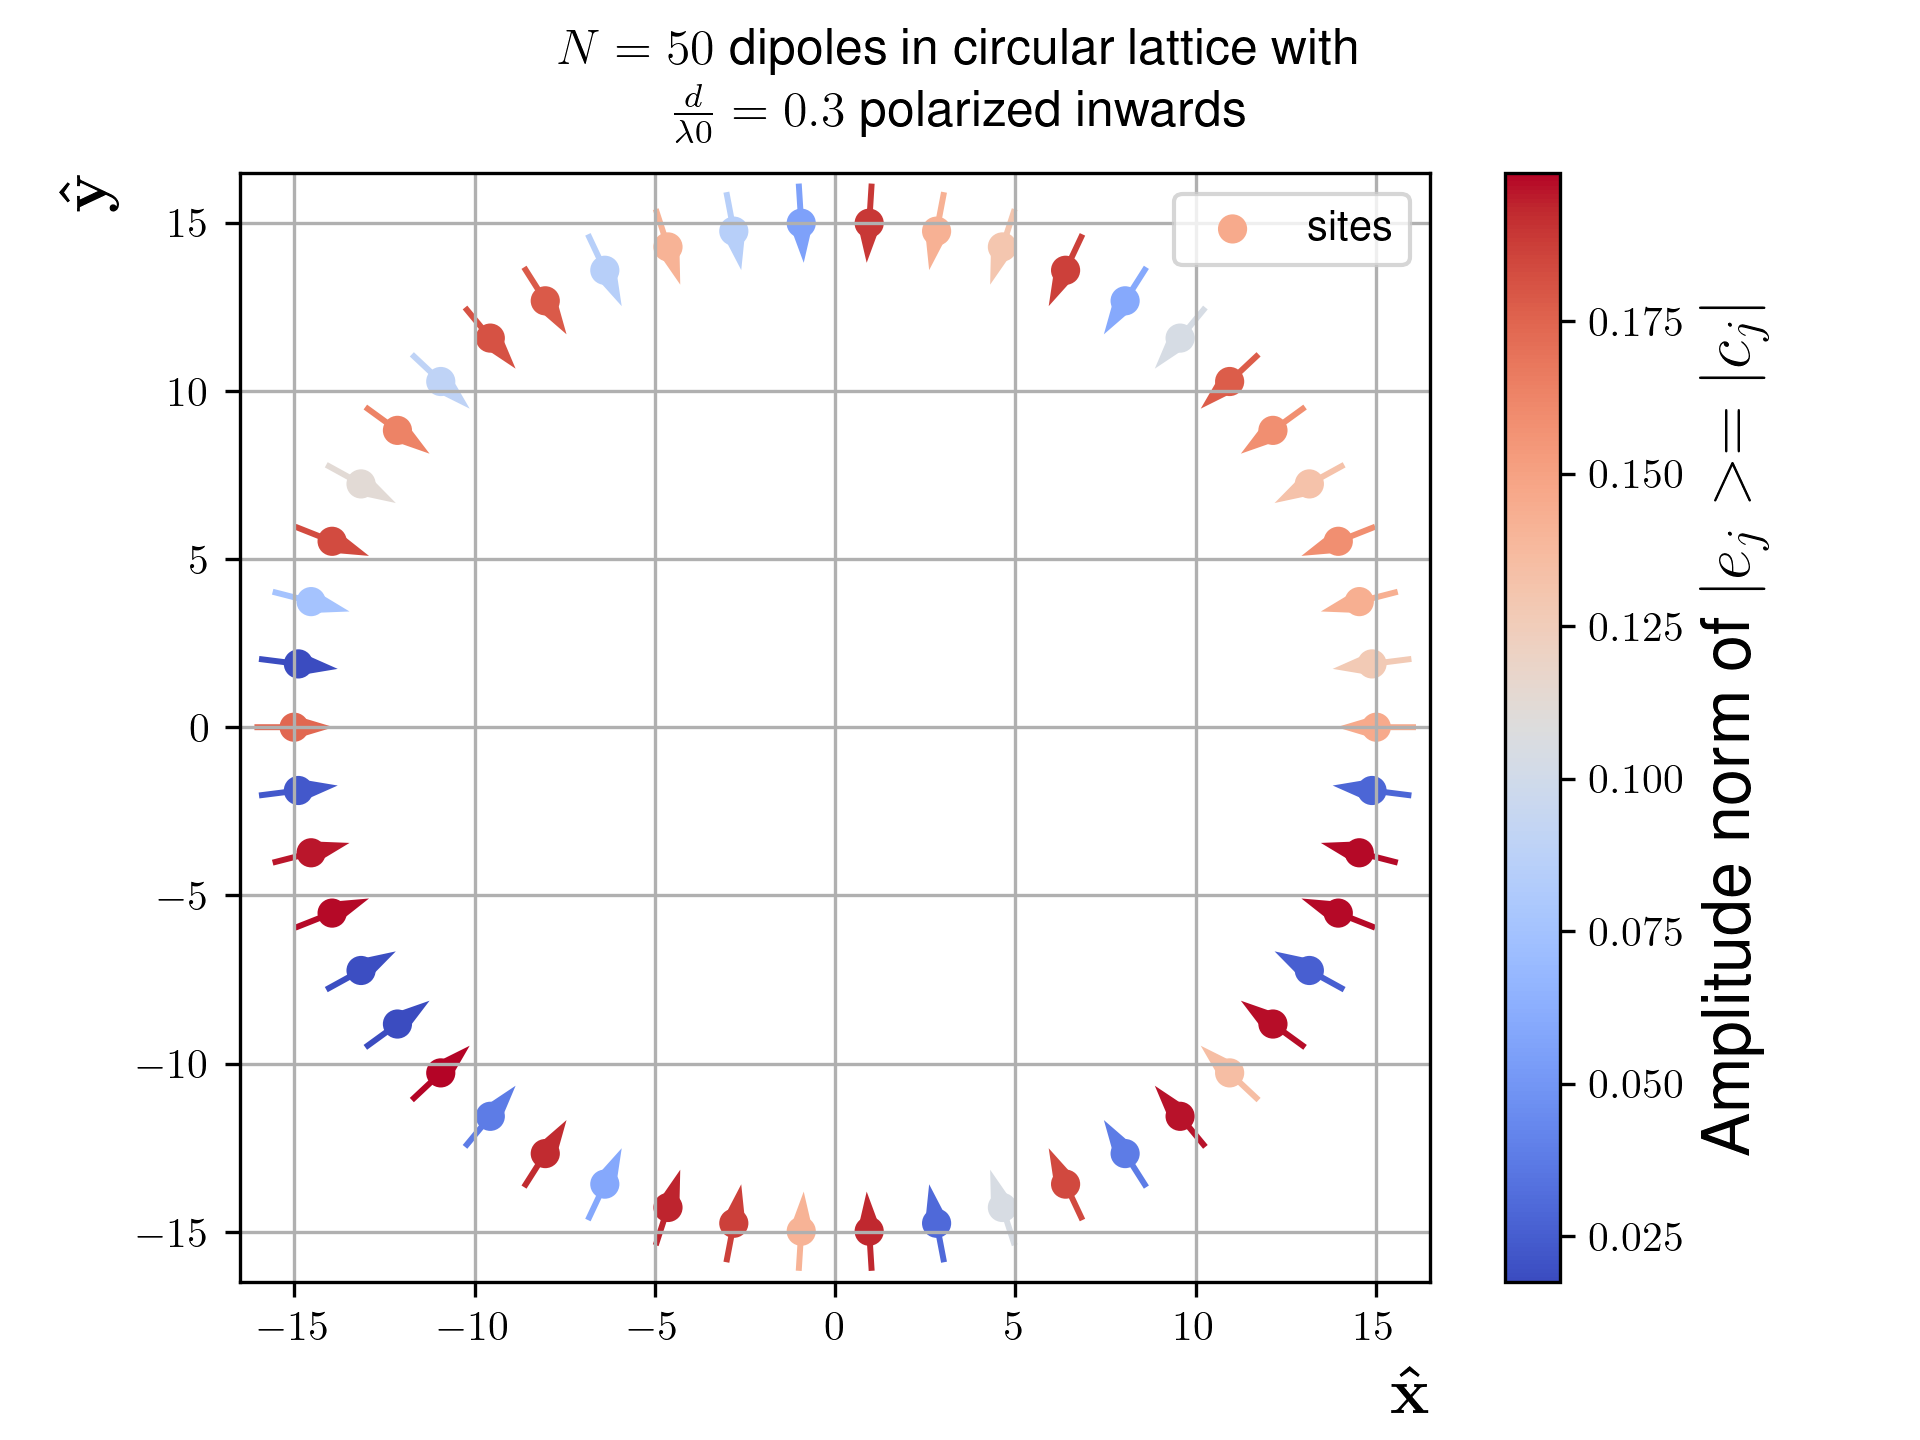
\includegraphics[width=\textwidth]{figs/dipoles_case_circular_inwards_lowest.png}
        \caption{}
        \label{fig:circular_inwards_lowest_eigenstate}
    \end{subfigure}
    \hfill
    \begin{subfigure}[b]{0.49\textwidth}
        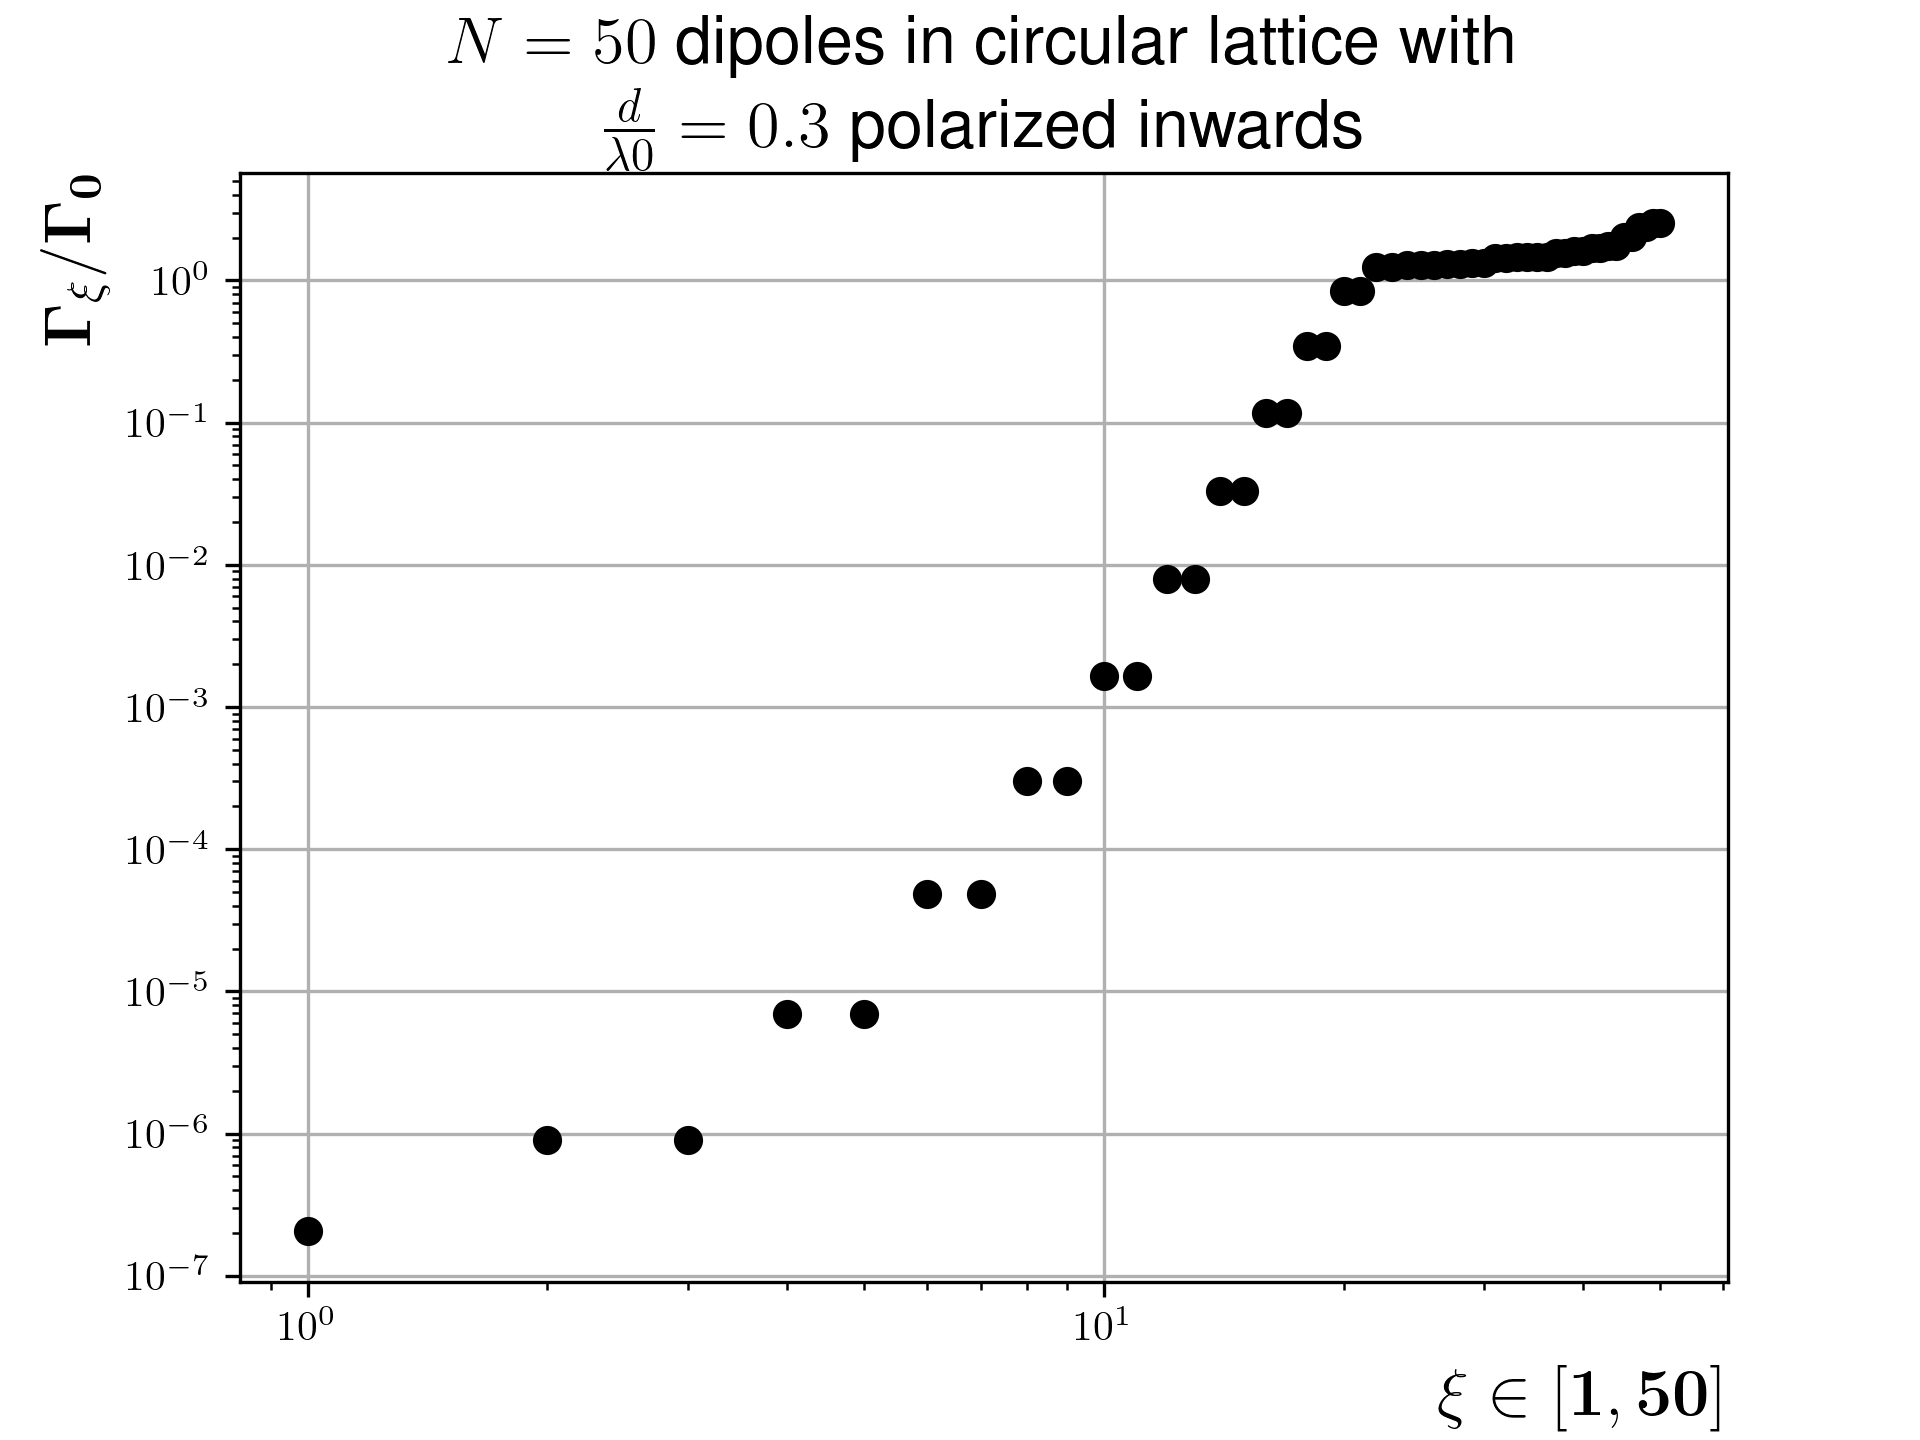
\includegraphics[width=\textwidth]{figs/case_circular_inwards_d_03.png}
        \caption{}
        \label{fig:circular_inwards_decayrates}
    \end{subfigure}
    \caption{}
    \label{fig:circular_inwards}
\end{figure}

\subsection{Negative decay rates}

For very small distances, e.g. $\frac{d}{\lambda0} = 0.00001$, the decay rates predicted by the diagonalization of the Hamiltonian can become negative, $a_\xi(t)=e^{-\Gamma_\xi t} a_\xi (0) \rightarrow e^{\Gamma_\xi t} a_\xi (0)$. This is of course unphysical. As seen, it would mean increase in probability. If the system initialized in a state with negative decay rate, the probability would become greater than 1. Why does it happen for very small interatomic distances? Remember, no assumption was made about the chosen transition. Choosing a microwave transition with optically trapped atoms would e.g. produce such circumstances (BUT MW TRANSITIONS ARE PHONONS?). 

Forudsigelser for N=2 tilfælde? Problemer! Sammenligning med Adrian N=3 kæde. Vidde på egenværdier gør det svært for algoritmen at være præcis, derfor skal der ikke så meget til, før vi havner på den forkerte side. TEORI?

\subsection{Outlook}\label{sec:outlook}

As mentioned in Section \ref{disc:linear_broken}, the broken linear chain has very different subradiant populated modes, compared to the unbroken case. A deeper investigation of this particular system could include an integration of the field-strength surrounding the system to see, where the broken chain radiates from. As noted, it is hypothesized that the linear chain radiates from the ends, so the apparent question is, if the broken chain radiates from corner as well? The field surrounding these systems in combination with time-evolution of the eigenstates could bring further insight in the radiative properties and wave-propagation throughout the systems. For atomic arrays in general to be a prospect for quantum information processing, in particular storing of states, the systems need a good trade-off between good coupling to the surrounding field, while not too strong. The circular chain does for instance not have any ends, from which the field may radiate, and this may prove difficult to retreive a state. In atomic ensembles, this problem has been overcome by coupling strongly to favored photon modes in a cavity (REF Yong), which yields efficient storage and retrieval protocols. As the strong coupling regime of CQED invalidates the Markovian approximations taken in Section \ref{sec:theory}, another approach must be investigated. 

One such approach is suggested in (REF Fayard), where a linear V-shaped chain of 3-level atoms are deployed. The extra level proves useful as a manipulator of collective excitations and can in theory be used to transfer a superradiant mode to a subradiant and vice-versa. This shopping between modes with desired properties can prove useful designing efficient protocols. 

Another example may be coupling of the atomic array to a wave-guide, as described in (REF Asenjo, Section IV). The framework developed by Grüner \& Welsch (REF) can be extended to include propagation in other media and guided modes. The guided modes of the wave-guide couple strongly to certain subradiant modes of the array, while the coupling to free space emission is still supressed. The lifetime of the subradiant states do however not improve much in this particular study, but the memory fidelity (i.e. store and retrieve) improves exponentially. A direction for further projects could be to simulate other geometrical configurations of arrays in combination with wave-guides. 

Further research in the track of this project could include more complex geometries. Suggestions include elliptic chains to study the decay rates dependencies of curvature and a helix-shaped array, which may incorporate features from the linear chain on the longitudinal axis and features from the circular chain in the radial axis. Complex geometries may yield interesting properties, but it is important to keep in mind that arranging atoms precisely below optical wavelengths is challenging, and increasing complexity in this manner could render the physical implementation outside of reach. 

Finally, another track continuing naturally from this project is multiexcitation states and their behaviour. As noted in (REF Asenjo), the multi-excitation states will, due to the spin-wave guided modes, exhibit fermionic behaviour, which impacts decay rates differently than for bosonic behaviour. 

\section{Conclusion}

\newpage
TODO: bibliography

\end{document}